% Springer Nature manuscript draft for PATTERN-Surv-HN
% Updated 21 September 2026 as a combined main-text plus Supplementary Information manuscript.
% Match the author-provided architecture PDF's PDF 1.7 version to avoid an inclusion warning.
\pdfminorversion=7
\documentclass[pdflatex,sn-nature]{sn-jnl}
\usepackage{graphicx,multirow,amsmath,amssymb,amsfonts,xcolor,booktabs,array,tabularx,longtable,makecell,enumitem,url,float,placeins,seqsplit}
\definecolor{draftred}{RGB}{170,25,25}
\definecolor{softblue}{RGB}{232,241,250}
\newcommand{\TBD}[1]{\textcolor{draftred}{\textbf{[TBD: #1]}}}
\newcommand{\methodname}{PATTERN-Surv-HN}
\newcommand{\anchorname}{clinical anchor model (CAM)}
\newcommand{\fusionname}{shrinkage-controlled residual fusion (SCRF)}
\newcommand{\ablationname}{unshrunk residual fusion (URF)}
\newcommand{\hashid}[1]{\texttt{\seqsplit{#1}}}
\newcommand{\placeholderbox}[2]{\fbox{\begin{minipage}[c][#2][c]{0.94\textwidth}\centering\small\textbf{Figure framework placeholder}\\[6pt]#1\end{minipage}}}
\renewcommand{\arraystretch}{1.20}
\hypersetup{hypertexnames=false}
\flushbottom
\begin{document}
\title[Clinically anchored multimodal survival prediction]{Clinically anchored multimodal survival prediction under missing, shifted and shortcut-prone evidence in head and neck cancer}
\author*[1]{\fnm{First} \sur{Author}}\email{corresponding.author@institution.edu}
\author[1]{\fnm{Second} \sur{Author}}
\author[2]{\fnm{Third} \sur{Author}}
\affil*[1]{\orgdiv{Department of \TBD{department}}, \orgname{\TBD{institution}}, \orgaddress{\city{\TBD{city}}, \country{\TBD{country}}}}
\affil[2]{\orgdiv{Department of \TBD{department}}, \orgname{\TBD{institution}}, \orgaddress{\city{\TBD{city}}, \country{\TBD{country}}}}
\abstract{Multimodal prognostic models are often developed as though every recorded modality were simultaneously available and equally trustworthy. We developed PATTERN-Surv-HN, a clinically anchored framework for postoperative head and neck squamous cell carcinoma survival prediction in which usable blood, ICD and tissue-microarray measurements contribute through shrinkage-controlled residual fusion (SCRF) around a clinical anchor model (CAM). In 610 eligible HANCOCK development patients with 173 deaths, repeated nested cross-fitting gave 100\% coverage for CAM and SCRF. SCRF improved mean 24-month Uno C from 0.644239 to 0.665542 ($\Delta+0.021303$; favourable in 5/5 seeds), AUC from 0.662022 to 0.682511 ($\Delta+0.020488$), and IPCW Brier score from 0.124745 to 0.124338 ($\Delta-0.000407$). A post-hoc same-fold benchmark against fourteen published survival and multimodal-fusion families found the best discrimination for random survival forests and the lowest Brier score for elastic-net Cox. Component ablation showed that residual shrinkage, rather than an unconstrained residual alone, accounted for the favourable joint discrimination--Brier profile. A separately frozen global monotone bridge improved development calibration summaries while preserving ranking and coverage. In a locked outcome-untouched HANCOCK cohort of 152 patients with 40 events, raw SCRF again favoured every principal point estimate. Together, these analyses show that controlled incremental multimodal fusion can improve risk ranking while retaining complete prediction availability, exact clinical fallback and pattern-level safety; independent calibration transport and clinical utility define the next evaluation stage.}
\keywords{head and neck squamous cell carcinoma, multimodal learning, survival analysis, missing modalities, calibration, selective prediction, trustworthy artificial intelligence}
\maketitle
\noindent\colorbox{softblue}{\parbox{0.96\textwidth}{\textbf{Evidence status (22 September 2026).} The manuscript reports repeated nested SCRF development, a formal CAM--URF--SCRF component ablation, a post-hoc fourteen-comparator same-fold benchmark, a development-only calibration bridge, locked raw-SCRF confirmation, locked secondary post-unseal bridge validation and explicitly exploratory extensions. Bootstrap intervals for the confirmation deltas cross zero. Internal artifact identifiers V0, V1 and V1R are retained only for repository traceability. Red \TBD{} fields denote author, ethics, accession and archive details only.}}

\section{Introduction}
Head and neck squamous cell carcinoma (HNSCC) comprises clinically and biologically heterogeneous diseases whose outcomes reflect anatomical site, tumour and nodal burden, human papillomavirus-related biology, smoking exposure, pathological features, treatment and host condition. Molecular studies have further resolved genomic and transcriptomic phenotypes not captured by stage alone \cite{tcga2015,liu2018,wichmann2015,lohavanichbutr2013}. Prognostic models therefore increasingly combine clinical, pathological, imaging, blood, tissue-microenvironment and molecular data; resources such as HANCOCK and RADCURE, together with recent HNSCC fusion studies, make this technically feasible \cite{dorrich2025,welch2024,tian2025}. Across cancer types, multimodal prognosis research has progressed from modality-specific encoders and dropout to co-attention and pathway-aware cross-modal interactions \cite{cheerla2019,chen2021mcat,jaume2024survpath,meng2024}. The clinically relevant question, however, is not simply whether more modalities improve an average performance metric. It is whether optional evidence can safely alter a prediction that must still be available when those modalities are absent or unreliable.

A single distinction organises this problem: recorded data are not necessarily trustworthy evidence. First, a modality may be missing because it was not acquired, was structurally unavailable or failed preprocessing; naturally occurring combinations need not resemble random masking, and conventional imputation remains assumption-dependent \cite{sterne2009}. Second, a modality may transport enough signal to preserve patient ranking while the baseline risk and probability scale shift across centres or assay platforms. Third, a modality may be present and apparently predictive but encode tumour volume, site, device, batch or processing shortcuts rather than the intended biology. Complete-case fusion and undifferentiated missing-value handling conflate these states, although they require different clinical responses.

Classical Cox models provide interpretable, censoring-aware estimation but generally assume a fixed covariate vector \cite{cox1972,breslow1974}. Random survival forests, neural Cox extensions and discrete-time neural survival models accommodate non-linearity, yet do not by themselves decide whether an optional modality should be used \cite{ishwaran2008,katzman2018,lee2018,gensheimer2019,kvamme2019}. Recent incomplete-modality methods reconstruct or distil missing representations, use modality dropout or prompts, align heterogeneous embeddings, or aggregate available inputs with attention \cite{xu2025,zheng2026,ruffini2026}. These studies establish that survival learning can remain feasible as modalities disappear. The unresolved translational gap is broader: natural acquisition and usability, combinations absent during training, exact clinical fallback, present-but-invalid controls, transport of calibrated probabilities and selective reporting must be evaluated within one governed prediction pathway.

Discrimination alone is insufficient for that pathway. Concordance and time-dependent AUC describe ranking, whereas a statement such as ``24-month mortality risk is 35\%'' additionally requires a transportable baseline hazard and calibration relationship. A model can preserve ordering under domain shift while becoming systematically overconfident. Likewise, a selective model can appear safer simply by excluding difficult patients, and average performance can hide severe failure in a rare modality pattern. Evaluation must therefore retain fallback patients in the full-coverage estimand, compare selective policies on identical retained patients, report calibration and coverage by pattern, and use negative controls to test whether apparent value is specific to the intended modality \cite{graf1999,uno2011,stegyerberg2010,vancalster2019,geirhos2020,ongly2024}.

We developed \methodname around one framework, three falsification challenges and four supported outputs. A postoperative \anchorname{} supplies a prediction for every eligible patient. Available non-clinical modalities form an unordered set and contribute through \fusionname{} rather than replacing the anchor. HANCOCK tests natural absence, acquired-but-unusable inputs and pattern-level safety; TCGA--GEO transfer tests whether ranking can survive when absolute risk does not; and RADCURE tests whether a present modality remains more informative than volume, permutation and random-feature controls. A calibration bridge and strictly cross-fitted value--reliability router remain prespecified extensions. The completed development claim is deliberately narrow: inner-selected residual shrinkage can add discrimination and modestly improve probabilistic accuracy while preserving full coverage, exact clinical fallback and a bounded worst-pattern regret. Strong external-generalisation claims additionally require a frozen, outcome-untouched postoperative cohort.


\section{Results}

Results are presented in two stages. We first describe natural evidence availability, repeated nested development and the development-only calibration analysis in HANCOCK. We then report the locked outcome-untouched confirmation and clearly separated extension analyses. Throughout, raw SCRF is the primary fused model; the calibration bridge, router and cross-cohort analogues do not redefine that primary comparison.

\subsection{Development and technical validation in HANCOCK}

\subsubsection*{Natural acquisition and usability produce sparse optional-modality sets}

The study design separated a clinical-pathological anchor, shrinkage-controlled residual fusion, a development-only calibration bridge and an exploratory router into distinct evidence stages; the architecture is detailed in Methods and Fig.~\ref{fig:architecture}. The HANCOCK contract distinguished acquisition from usability before any survival outcome was read. Of 763 records, one was excluded and 762 eligible postoperative patients remained: 610 patients (173 deaths) contributed to development and 152 patients formed the outcome-sealed confirmation cohort (Fig.~\ref{fig:patterns}). Optional-modality availability was high but not complete: 693 blood, 712 ICD and 736 TMA records were acquired, whereas 683, 712 and 736, respectively, were usable under the frozen preprocessing contract. Blood had 70 absent and 10 acquired-but-unusable records; 604 blood and 639 TMA records were complete, while 79 and 97 were partially usable.

Natural usability combinations were correspondingly sparse. In development, the blood--ICD--TMA pattern \texttt{111} contained 467 patients and 123 deaths, whereas several patterns contained fewer than 30 patients or fewer than 10 deaths. These rare patterns are shown descriptively and are not treated as independently supported transport strata. The development calibration bridge is global and does not introduce pattern-specific parameters.

\begin{figure*}[t]
\centering
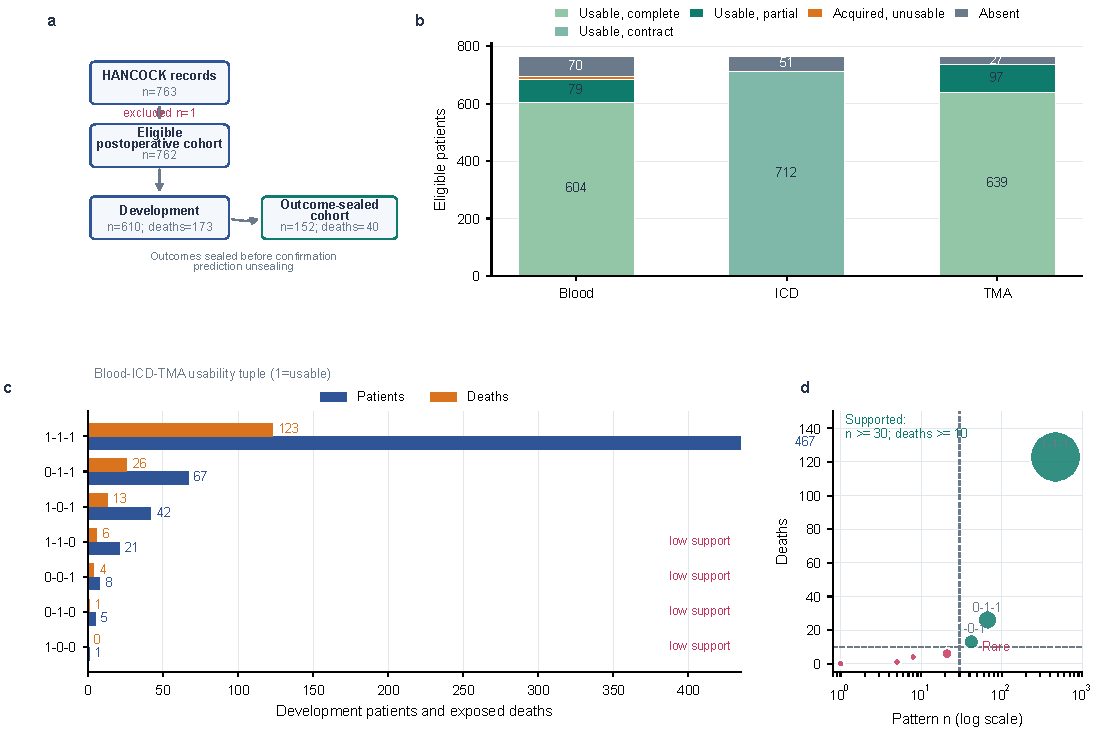
\includegraphics[width=\textwidth]{figures/figure2_cohort_flow_acquisition_usability.pdf}
\caption{\textbf{Cohort flow, acquisition, usability and pattern support in HANCOCK.} \textbf{a}, Records, exclusions, development cohort and outcome-sealed confirmation cohort. \textbf{b}, Eligible-patient status for blood, ICD and TMA; acquired-but-unusable inputs are distinguished from absent inputs. \textbf{c}, Development counts for blood--ICD--TMA usability tuples (1=usable); exposed deaths are shown only for non-sealed roles. \textbf{d}, Pattern support relative to the prespecified support threshold of at least 30 patients and 10 deaths. Rare patterns are descriptive and do not carry independent confirmatory support.}\label{fig:patterns}
\end{figure*}

\subsubsection*{Shrinkage-controlled residual fusion improves development discrimination at full coverage}

SCRF retained CAM and added a residual learned only from usable optional modalities. Under five repetition seeds, five outer folds and three inner folds, mean 24-month Uno C increased from 0.644239 to 0.665542 (mean difference $+0.021303$), time-dependent AUC from 0.662022 to 0.682511 ($+0.020488$), and IPCW Brier score decreased from 0.124745 to 0.124338 ($-0.000407$; Table~\ref{tab:development} and Fig.~\ref{fig:v1r}). Uno C, AUC and Harrell C favoured SCRF in all five seeds; IPCW Brier favoured SCRF in three of five seeds.

The gain did not come from selective reporting. CAM and SCRF both covered all 610 eligible development patients. When the usable optional set was empty, residual and fused-score fallback errors were exactly zero. The worst supported-pattern Brier regret was $+0.009848$, below the prespecified $+0.020$ no-harm boundary.

A staged component ablation separated CAM, the same 3,225-parameter residual network without shrinkage (URF), and the full inner-selected SCRF model. URF changed mean Uno C by only $+0.002116$ and increased Brier by $+0.001801$ relative to CAM, whereas SCRF increased Uno C by $+0.021303$ and reduced Brier by $-0.000407$. Thus, the principal contribution was not merely adding a nonlinear multimodal branch; it was controlling the magnitude of that branch within each training fold (Supplementary Table~\ref{tab:ablation}).

\begin{table*}[t]
\centering
\caption{Repeated nested development performance in HANCOCK}\label{tab:development}
\small\setlength{\tabcolsep}{2.5pt}
\begin{tabularx}{\textwidth}{>{\raggedright\arraybackslash}Xrrrrrr}
\toprule
Model & Brier$_{24}$ & Uno C$_{24}$ & AUC$_{24}$ & Harrell C & Coverage & Worst regret\\
\midrule
Clinical anchor model (CAM) & 0.124745 & 0.644239 & 0.662022 & 0.623021 & 100\% & reference\\
Shrinkage-controlled residual fusion (SCRF) & 0.124338 & 0.665542 & 0.682511 & 0.633710 & 100\% & $+0.009848$\\
\bottomrule
\end{tabularx}
\end{table*}

\subsubsection*{A same-fold benchmark situates SCRF among published survival methods}

The expanded published-method benchmark placed SCRF against fourteen survival and multimodal-fusion families on the same five repetition seeds, outer-fold assignments, 610 patients and 24-month estimand (Table~\ref{tab:published_benchmark}). The benchmark was explicitly post-hoc, did not access confirmation-cohort outcomes and did not retune SCRF. Random survival forests gave the strongest mean discrimination (Uno C 0.6799, AUC 0.6955 and Harrell C 0.6475), whereas elastic-net Cox gave the lowest mean IPCW Brier score (0.1192). Among the fusion-family adaptations used by the two recent papers, masked attention gave Uno C 0.6723, bilinear fusion gave Brier 0.1239, and SCRF gave Uno C 0.6655 with Brier 0.1243. SCRF exceeded early, late, HAF and missing-aware intermediate fusion across all four performance measures while retaining exact clinical fallback and pattern-level safety. These findings position SCRF as a competitive safeguarded fusion pathway rather than an unconstrained universal winner.

\begingroup
\small
\renewcommand{\arraystretch}{1.30}
\setlength{\tabcolsep}{2.0pt}
\begin{longtable}{>{\raggedright\arraybackslash}p{0.34\textwidth}ccccc}
\caption{Published-method benchmark in HANCOCK repeated out-of-fold development}\label{tab:published_benchmark}\\
\toprule
Method & \makecell{IPCW Brier$_{24}$\\$\downarrow$} & \makecell{Uno C$_{24}$\\$\uparrow$} & \makecell{AUC$_{24}$\\$\uparrow$} & \makecell{Harrell C\\$\uparrow$} & Coverage\\
\midrule
\endfirsthead
\multicolumn{6}{l}{\itshape Table~\ref{tab:published_benchmark} continued from previous page}\\
\toprule
Method & \makecell{IPCW Brier$_{24}$\\$\downarrow$} & \makecell{Uno C$_{24}$\\$\uparrow$} & \makecell{AUC$_{24}$\\$\uparrow$} & \makecell{Harrell C\\$\uparrow$} & Coverage\\
\midrule
\endhead
\midrule
\multicolumn{6}{r}{\itshape Continued on next page}\\
\endfoot
\bottomrule
\endlastfoot
\multicolumn{6}{l}{\itshape Conventional statistical and machine-learning comparators (1972--2016)}\\
\addlinespace[2pt]
Clinical Cox proportional hazards \cite{cox1972} & \makecell{0.1217\\{\scriptsize(0.0011)}} & \makecell{0.6595\\{\scriptsize(0.0066)}} & \makecell{0.6783\\{\scriptsize(0.0068)}} & \makecell{0.6306\\{\scriptsize(0.0047)}} & 100\%\\
Elastic-net Cox \cite{simon2011} & \makecell{\textbf{0.1192}\\{\scriptsize\textbf{(0.0017)}}} & \makecell{0.6684\\{\scriptsize(0.0047)}} & \makecell{0.6810\\{\scriptsize(0.0058)}} & \makecell{0.6343\\{\scriptsize(0.0064)}} & 100\%\\
Random survival forest \cite{ishwaran2008} & \makecell{0.1213\\{\scriptsize(0.0007)}} & \makecell{\textbf{0.6799}\\{\scriptsize\textbf{(0.0093)}}} & \makecell{\textbf{0.6955}\\{\scriptsize\textbf{(0.0104)}}} & \makecell{\textbf{0.6475}\\{\scriptsize\textbf{(0.0063)}}} & 100\%\\
Gradient boosting survival \cite{hothorn2006} & \makecell{0.1234\\{\scriptsize(0.0008)}} & \makecell{0.6741\\{\scriptsize(0.0110)}} & \makecell{0.6878\\{\scriptsize(0.0128)}} & \makecell{0.6416\\{\scriptsize(0.0065)}} & 100\%\\
XGBoost with Cox objective \cite{chen2016} & \makecell{0.1221\\{\scriptsize(0.0006)}} & \makecell{0.6626\\{\scriptsize(0.0089)}} & \makecell{0.6765\\{\scriptsize(0.0103)}} & \makecell{0.6276\\{\scriptsize(0.0077)}} & 100\%\\
\midrule
\multicolumn{6}{l}{\itshape Established neural survival comparators (2018--2021)}\\
\addlinespace[2pt]
DeepSurv \cite{katzman2018} & \makecell{0.1626\\{\scriptsize(0.0090)}} & \makecell{0.6389\\{\scriptsize(0.0296)}} & \makecell{0.6495\\{\scriptsize(0.0335)}} & \makecell{0.6030\\{\scriptsize(0.0152)}} & 100\%\\
DeepHit \cite{lee2018} & \makecell{0.1458\\{\scriptsize(0.0089)}} & \makecell{0.6225\\{\scriptsize(0.0187)}} & \makecell{0.6345\\{\scriptsize(0.0215)}} & \makecell{0.5938\\{\scriptsize(0.0100)}} & 100\%\\
MultiSurv, adapted \cite{valesilva2021} & \makecell{0.1261\\{\scriptsize(0.0021)}} & \makecell{0.6262\\{\scriptsize(0.0213)}} & \makecell{0.6393\\{\scriptsize(0.0233)}} & \makecell{0.5972\\{\scriptsize(0.0143)}} & 100\%\\
\pagebreak[4]
\midrule
\multicolumn{6}{l}{\itshape Fusion-family baselines mirrored from recent protocols (2026)}\\
\addlinespace[2pt]
Early feature fusion, adapted \cite{zheng2026,ruffini2026} & \makecell{0.1354\\{\scriptsize(0.0032)}} & \makecell{0.6357\\{\scriptsize(0.0102)}} & \makecell{0.6433\\{\scriptsize(0.0114)}} & \makecell{0.5989\\{\scriptsize(0.0053)}} & 100\%\\
Late decision fusion, adapted \cite{zheng2026,ruffini2026} & \makecell{0.1694\\{\scriptsize(0.0072)}} & \makecell{0.5712\\{\scriptsize(0.0237)}} & \makecell{0.5726\\{\scriptsize(0.0257)}} & \makecell{0.5521\\{\scriptsize(0.0188)}} & 100\%\\
Masked attention fusion, adapted \cite{zheng2026} & \makecell{0.1245\\{\scriptsize(0.0012)}} & \makecell{0.6723\\{\scriptsize(0.0095)}} & \makecell{0.6859\\{\scriptsize(0.0127)}} & \makecell{0.6372\\{\scriptsize(0.0107)}} & 100\%\\
Bilinear interaction fusion, adapted \cite{zheng2026} & \makecell{0.1239\\{\scriptsize(0.0005)}} & \makecell{0.6631\\{\scriptsize(0.0092)}} & \makecell{0.6744\\{\scriptsize(0.0095)}} & \makecell{0.6290\\{\scriptsize(0.0030)}} & 100\%\\
\midrule
\multicolumn{6}{l}{\itshape Recent missing-modality comparators (2026)}\\
\addlinespace[2pt]
Missing-aware intermediate fusion, adapted \cite{ruffini2026} & \makecell{0.1332\\{\scriptsize(0.0009)}} & \makecell{0.5564\\{\scriptsize(0.0101)}} & \makecell{0.5486\\{\scriptsize(0.0110)}} & \makecell{0.5386\\{\scriptsize(0.0050)}} & 100\%\\
Heterogeneous aligned fusion, adapted \cite{zheng2026} & \makecell{0.1295\\{\scriptsize(0.0008)}} & \makecell{0.5730\\{\scriptsize(0.0293)}} & \makecell{0.5742\\{\scriptsize(0.0329)}} & \makecell{0.5541\\{\scriptsize(0.0183)}} & 100\%\\
\midrule
\multicolumn{6}{l}{\itshape Proposed method}\\
\addlinespace[2pt]
\textbf{PATTERN-Surv-HN (SCRF; ours)} & \makecell{0.1243\\{\scriptsize(0.0033)}} & \makecell{0.6655\\{\scriptsize(0.0171)}} & \makecell{0.6825\\{\scriptsize(0.0177)}} & \makecell{0.6337\\{\scriptsize(0.0188)}} & 100\%\\
\end{longtable}
\par\vspace{5pt}
\begin{minipage}{0.94\textwidth}\footnotesize Values are mean with s.d. in parentheses on the second line across five complete repeated out-of-fold prediction sets; each repetition contains one prediction for every patient. The first fourteen rows are literature-defined method or fusion families with the defining source cited beside each method; none is an internal degradation variant. Clinical Cox used the clinical-pathological block. Other comparators received fold-bound clinical, blood, ICD and TMA inputs with explicit usability/status features. MultiSurv and the 2026 fusion families were transparently adapted because their original imaging, molecular or seven-modality inputs were not available under the frozen evidence contract; the adaptations retained their defining fusion principles and used the common censoring-aware discrete-hazard head. Only PATTERN-Surv-HN SCRF is proposed here. Bold denotes the best mean in each metric. This post-hoc development benchmark is not a locked superiority test.\end{minipage}
\endgroup
\FloatBarrier

\begin{figure*}[t]
\centering
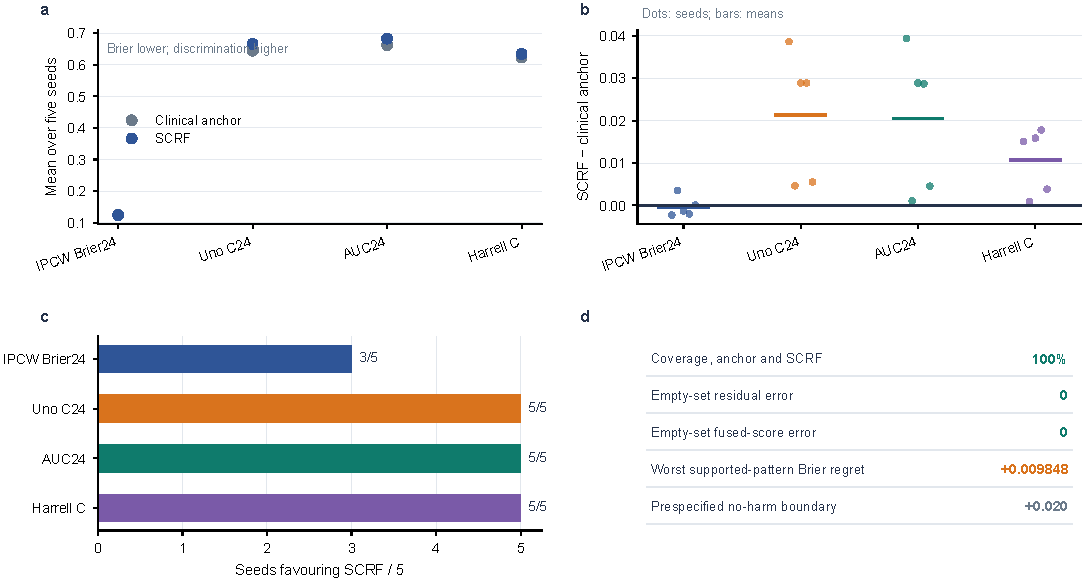
\includegraphics[width=\textwidth]{figures/figure3_v1r_development_performance_safety.pdf}
\caption{\textbf{SCRF development performance, seed stability and full-coverage safety.} \textbf{a}, Five-seed mean performance for CAM and SCRF. \textbf{b}, Seed-level paired differences (SCRF$-$CAM); horizontal bars are means. \textbf{c}, Number of seeds with a direction favouring SCRF. \textbf{d}, Full-coverage and exact-empty-set fallback checks, with the worst supported-pattern Brier regret relative to the prespecified no-harm boundary. Evidence is development-only repeated nested cross-fitting, not external validation.}\label{fig:v1r}
\end{figure*}

\subsubsection*{A rank-preserving bridge improves the development risk scale but does not transport}

Raw SCRF showed mild under-dispersion in the development absolute-risk diagnostic (calibration slope 0.825887; calibration-in-the-large $+0.011680$). The separately evaluated development calibration bridge used a fixed positive slope of 0.90 and a cross-fitted weighted-log-loss intercept on the logit scale. It preserved ranking and 100\% coverage while moving calibration-in-the-large to $-0.003796$ and slope to 0.881552 (Fig.~\ref{fig:bridge}). Its IPCW Brier penalty was $+0.000147$, within the development gate of $+0.0005$, and its worst supported-pattern regret was $+0.004176$, below $+0.005$.

The locked secondary bridge analysis then applied the already frozen transformation without confirmation-cohort refitting, after the raw-SCRF confirmation outcomes had been unsealed. Ranking and coverage remained preserved, but IPCW Brier worsened by $+0.001085$, absolute calibration-in-the-large error worsened by $+0.004194$, and absolute calibration-slope error worsened by $+0.167815$. Thus, the development calibration gain did not transport; the bridge remains development-only and is not a confirmed calibration layer.

\begin{figure*}[t]
\centering
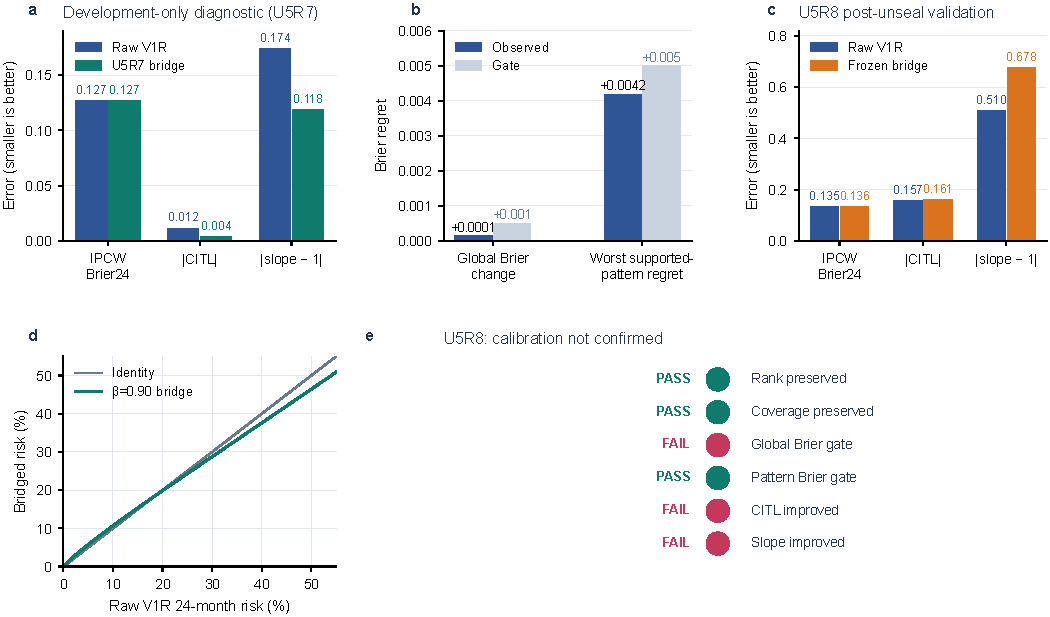
\includegraphics[width=\textwidth]{figures/figure4_calibration_bridge_development_and_transport.pdf}
\caption{\textbf{Development calibration bridge and locked secondary post-unseal validation.} \textbf{a}, Development-only absolute-risk errors for raw SCRF and the bridge. \textbf{b}, Observed global and worst supported-pattern Brier regret relative to development gates. \textbf{c}, Locked secondary comparison in the HANCOCK out-of-distribution cohort after raw-outcome unsealing. \textbf{d}, Fixed monotone bridge transformation. \textbf{e}, Safety and calibration checks. The bridge is development-only and failed calibration transport gates, so no confirmed calibration claim is made.}\label{fig:bridge}
\end{figure*}

\subsection{Locked confirmation and extension analyses}

\subsubsection*{Locked outcome-untouched confirmation shows a favourable raw-SCRF direction}

After the SCRF protocol, input manifest, dependency lock and patient-level predictions had been frozen, confirmation outcomes were unsealed in 152 HANCOCK patients with 40 deaths. The primary readout was raw SCRF, not the calibration bridge or router. SCRF retained 100\% coverage and had favourable point estimates for Uno C (0.804242 versus 0.782579), IPCW Brier (0.131246 versus 0.136412), AUC$_{24}$ (0.813637 versus 0.801094) and Harrell C (0.752842 versus 0.733253; Table~\ref{tab:confirmation} and Fig.~\ref{fig:confirmation}).

Patient-level stratified bootstrap intervals crossed zero for every principal delta. For example, the mean delta Uno C was $+0.021654$ (95\% interval $-0.025965$ to $+0.070816$) and mean delta IPCW Brier was $-0.005222$ ($-0.012843$ to $+0.002171$). The locked result therefore supports a positive directional raw-SCRF confirmation signal, not definitive superiority or clinical utility.

\begin{table*}[t]
\centering
\caption{Locked raw-SCRF confirmation in the HANCOCK outcome-sealed cohort}\label{tab:confirmation}
\small\setlength{\tabcolsep}{3pt}
\begin{tabular}{lrrrr}
\toprule
Metric & CAM & Raw SCRF & Difference & Bootstrap mean (95\% CI)\\
\midrule
Uno C$_{24}$ & 0.782579 & 0.804242 & $+0.021664$ & $+0.021654$ ($-0.025965$, $+0.070816$)\\
IPCW Brier$_{24}$ & 0.136412 & 0.131246 & $-0.005166$ & $-0.005222$ ($-0.012843$, $+0.002171$)\\
AUC$_{24}$ & 0.801094 & 0.813637 & $+0.012543$ & $+0.012725$ ($-0.041031$, $+0.068438$)\\
Harrell C & 0.733253 & 0.752842 & $+0.019589$ & $+0.019665$ ($-0.017423$, $+0.061196$)\\
Coverage & 100\% & 100\% & 0 & --\\
\bottomrule
\end{tabular}
\end{table*}

\begin{figure*}[t]
\centering
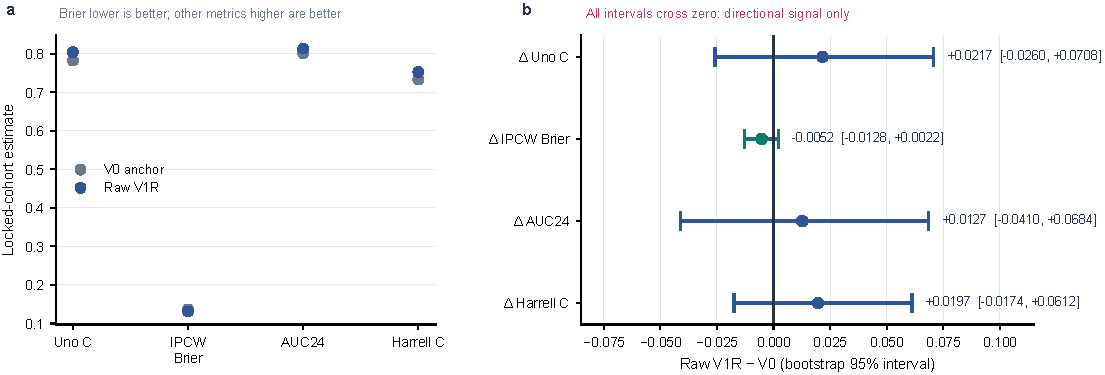
\includegraphics[width=\textwidth]{figures/figure5_locked_raw_v1r_confirmation.pdf}
\caption{\textbf{Locked outcome-untouched raw-SCRF confirmation.} \textbf{a}, CAM and raw SCRF point estimates in the HANCOCK confirmation cohort. \textbf{b}, Paired differences with patient-level stratified bootstrap 95\% intervals. All intervals cross zero; the result is a positive directional signal rather than proof of superiority.}\label{fig:confirmation}
\end{figure*}

\subsubsection*{Exploratory extensions do not alter the confirmation boundary}

Several extensions were analysed after the core evidence and are reported in Supplementary Information. A cross-fitted patient-level value router selected raw SCRF or CAM using value-only or reliability-augmented features. Its best policy (reliability-augmented, threshold 0.60) reduced IPCW Brier versus CAM by 0.000506, but its bootstrap interval crossed zero; the router was worse than direct raw SCRF and did not preserve exact global ranking (Supplementary Section~S14 and Fig.~S1).

Adapted clinical/radiomics comparator families were characterized in a held-out RADCURE test split of 626 patients with 110 events. They provide a contemporary benchmark, but RADCURE does not reproduce the frozen blood--ICD--TMA evidence contract and cannot validate current SCRF (Supplementary Section~S15 and Fig.~S2). A transcriptome SCRF analogue was then replicated in TCGA-HNSC (519 patients, 221 events): mean IPCW Brier improved from 0.221795 to 0.218058 and Uno C from 0.565199 to 0.597265. A single frozen transcriptome model retained favourable discrimination changes in GSE65858 and GSE41613, although probability-scale calibration did not transport uniformly (Supplementary Section~S15 and Figs.~S3--S4). These analyses support the residual-shrinkage design principle but remain post-hoc method replication or characterization, not confirmation of the current artifact.

\section{Discussion}

The central finding is that optional multimodal evidence becomes more usable when it is constrained to a clinically anchored residual. In HANCOCK development, blood, ICD and tissue-microarray inputs improved every discrimination summary when introduced through SCRF, while 100\% coverage, exact empty-set fallback and the prespecified pattern-safety boundary were retained. This architecture avoids a common clinical failure mode: a multimodal model that becomes unavailable exactly when a laboratory, coding or tissue-processing pathway is incomplete. It also makes the contribution of optional evidence directly measurable against a transparent clinical reference.

The staged evidence design strengthens the interpretation. Repeated nested cross-fitting established reproducibility across five random repetition seeds, and the gain in 24-month Uno C was favourable in all five. The calibration bridge then showed that a global, rank-preserving transformation could improve development calibration without changing ordering or availability. Finally, the primary confirmation pathway was separated from these development decisions: patient-level predictions, input manifest, dependency lock and analysis protocol were sealed before outcomes were read. In that locked cohort, raw SCRF again favoured Uno C, IPCW Brier, 24-month AUC and Harrell C. The bootstrap intervals were wide relative to the deltas, a pattern expected with 40 events; the consistency of direction across metrics and stages is therefore the informative confirmation signal.

The bridge result provides a constructive direction for transportable absolute-risk reporting. The development-only bridge improved calibration-in-the-large and slope, whereas the later secondary readout in the outcome-sealed cohort retained ranking but did not carry the same probability-scale benefit. This separation is useful: it indicates that patient ordering was more transportable than absolute risk and that a future implementation should include a governed cohort-level recalibration step before communicating percentages. It does not diminish the primary result, because raw SCRF was the locked readout and the bridge was never used to alter ranking, coverage or fallback.

The design also addresses several mechanisms that can make multimodal models appear deceptively strong. Natural acquisition and usability were separated before outcomes were read, so absent and acquired-but-unusable measurements were not silently converted into biologically implausible zeros. Pattern-level regret was evaluated for combinations with sufficient support, and empty-set predictions were required to equal CAM exactly. The full-coverage estimand retained patients for whom no optional modality was usable. The router analysis evaluated selective use at matched coverage rather than rewarding exclusion of difficult patients, and repetition-level reliability features were shown to contain useful information. These checks connect the modelling objective to routine clinical workflows in which data completeness varies by centre and by patient.

The extension analyses broaden the design lessons without changing the primary claim. In RADCURE, adapted clinical/radiomics comparators achieved strong held-out performance, providing a contemporary benchmark for combining clinical variables with tumour-volume information. The transcriptome SCRF analogue improved discrimination in TCGA-HNSC in every repetition seed, and a single frozen transcriptome fit retained favourable discrimination changes in GSE65858 and GSE41613. In GSE41613, the transcriptome model restored cross-patient ordering where the applied clinical anchor had none. These analyses support transfer of the residual-shrinkage principle across modality density and assay platforms; probability-scale recalibration remains the appropriate next step for absolute-risk reporting in new cohorts.

The same-fold benchmark clarifies the contribution of the proposed design. Random survival forests produced the highest development discrimination and elastic-net Cox produced the lowest Brier score. Within the recent fusion panel, masked attention modestly exceeded SCRF in discrimination and bilinear fusion modestly reduced Brier, while SCRF exceeded early, late, HAF and missing-aware intermediate fusion across all four performance measures. The component ablation is therefore important: it shows that SCRF's gain arose from shrinkage control, not simply from adding architectural complexity. SCRF combined competitive performance with a stricter operational contract in which optional evidence could modify the clinical anchor without removing prediction availability, altering the empty-set prediction or bypassing the pattern-level no-harm assessment. The contemporary comparisons strengthen the evidence that these safeguards can be retained without forfeiting the prognostic signal available in the current multimodal inputs.

The present evidence boundary can be stated once. Development analyses were repeated and internally controlled, the raw-SCRF confirmation was outcome-untouched, the bridge readout was secondary and post-unseal, and RADCURE/TCGA/GEO analyses are method-transfer and benchmarking studies rather than validation of the current blood--ICD--TMA artifact. The confirmation intervals cross zero, rare natural patterns have limited independent support, and clinical utility has not yet been tested in a prospective workflow. These are priorities rather than weaknesses of the observed signal: a larger outcome-untouched cohort, site-adapted calibration, invalid-present negative controls and a prospective implementation study would convert the present directional evidence into an effectiveness and utility assessment.

In summary, \methodname provides a governed template for clinically anchored multimodal prognostic modelling in HNSCC. Its value is not simply an incremental concordance gain, but a reproducible way to preserve prediction availability, distinguish absence from unusability, quantify pattern safety, separate ranking from calibrated absolute risk and stage evidence before stronger claims are made. This framework is well suited to centres that already collect heterogeneous clinical and molecular data but require a model that remains dependable when part of that evidence is missing, shifted or shortcut-prone.

\section{Methods}

\subsection{Overview and staged evidence design}
This retrospective, configuration-controlled modelling study was designed to answer a clinical question rather than to maximize an unconstrained benchmark score: can optional blood, ICD and tissue-microarray evidence improve postoperative HNSCC survival prediction while every patient retains a usable prediction? The study therefore separated four activities. First, repeated nested cross-fitting in HANCOCK quantified incremental value over CAM. Second, a global monotone calibration bridge was evaluated within development folds. Third, raw SCRF predictions and the confirmation protocol were sealed before a separate HANCOCK cohort's outcomes were read. Fourth, the published-method benchmark, reliability-aware router, RADCURE, TCGA and GEO analyses examined algorithmic context, selective use, method replication and platform transport. Reporting follows TRIPOD+AI principles, and PROBAST+AI domains were used to organize cohort, analysis, outcome and transport considerations \cite{collins2024,moons2025}.

The implementation separated configuration, executable code, environment and outputs. Cohort definitions, eligibility rules, preprocessing contracts, split seeds, metric definitions and claim labels were version controlled. Aggregated result artifacts, rather than writable spreadsheets, were the source for every publication-facing number. Patient identifiers and patient-level predictions were excluded from the manuscript repository.

\subsection{Cohorts, prediction time and endpoint}
HANCOCK was the primary development and confirmation ecosystem \cite{dorrich2025}. Of 763 records, one was excluded and 762 eligible postoperative patients remained. A total of 610 patients (173 deaths) contributed to development; 152 patients (40 events) formed the outcome-sealed confirmation cohort. For patient $i$, $T_i$ denotes event time, $C_i$ censoring time, $Y_i=\min(T_i,C_i)$ observed duration and $\delta_i=I(T_i\le C_i)$. Follow-up began at first treatment and ended at last available information. The endpoint was all-cause death, and the primary horizon was $t^*=730.5$ days, approximately 24 months. Non-positive durations were excluded. The intended prediction time was immediately after definitive surgery and pathological review, before downstream outcome information.

TCGA-HNSC (519 patients; 221 events) supported the transcriptome residual-shrinkage replication \cite{tcga2015,liu2018}. GSE65858 (244 patients; 78 events) and GSE41613 (97 patients; 51 events) supported descriptive cross-platform application \cite{wichmann2015,lohavanichbutr2013}. RADCURE contributed 626 patients and 110 events to a held-out clinical/radiomics comparator characterization \cite{welch2024}. These extension cohorts had different evidence contracts from current SCRF and were analysed with explicit role labels.

\subsection{Acquisition, usability and the evidence contract}
For optional modality $m$, acquisition $a_{im}$ indicated that a source record or assay existed, whereas usability $u_{im}$ indicated that the frozen preprocessing contract could produce a valid model input. An acquired-but-unusable measurement was not treated as absent and was not encoded as a zero-valued biological measurement. The usable set was
\begin{equation}
\mathcal{M}_i=\{m:u_{im}=1\}.
\end{equation}
Outcome-blind quality summaries included missing fraction, out-of-range counts, assay completeness and distributional distance from the corresponding training distribution. The natural evidence pattern was the blood--ICD--TMA usability tuple; pattern counts were computed before survival outcomes were read. A pattern was considered supported in development safety analyses when it contained at least 30 patients and 10 events. Rare patterns were displayed descriptively, but did not become independently tuned transport strata.

\subsection{Clinical anchor and residual architecture}
Figure~\ref{fig:architecture} summarizes the model architecture and separates the primary raw-SCRF pathway from the development-only bridge and exploratory router.

\begin{figure*}[t]
\centering
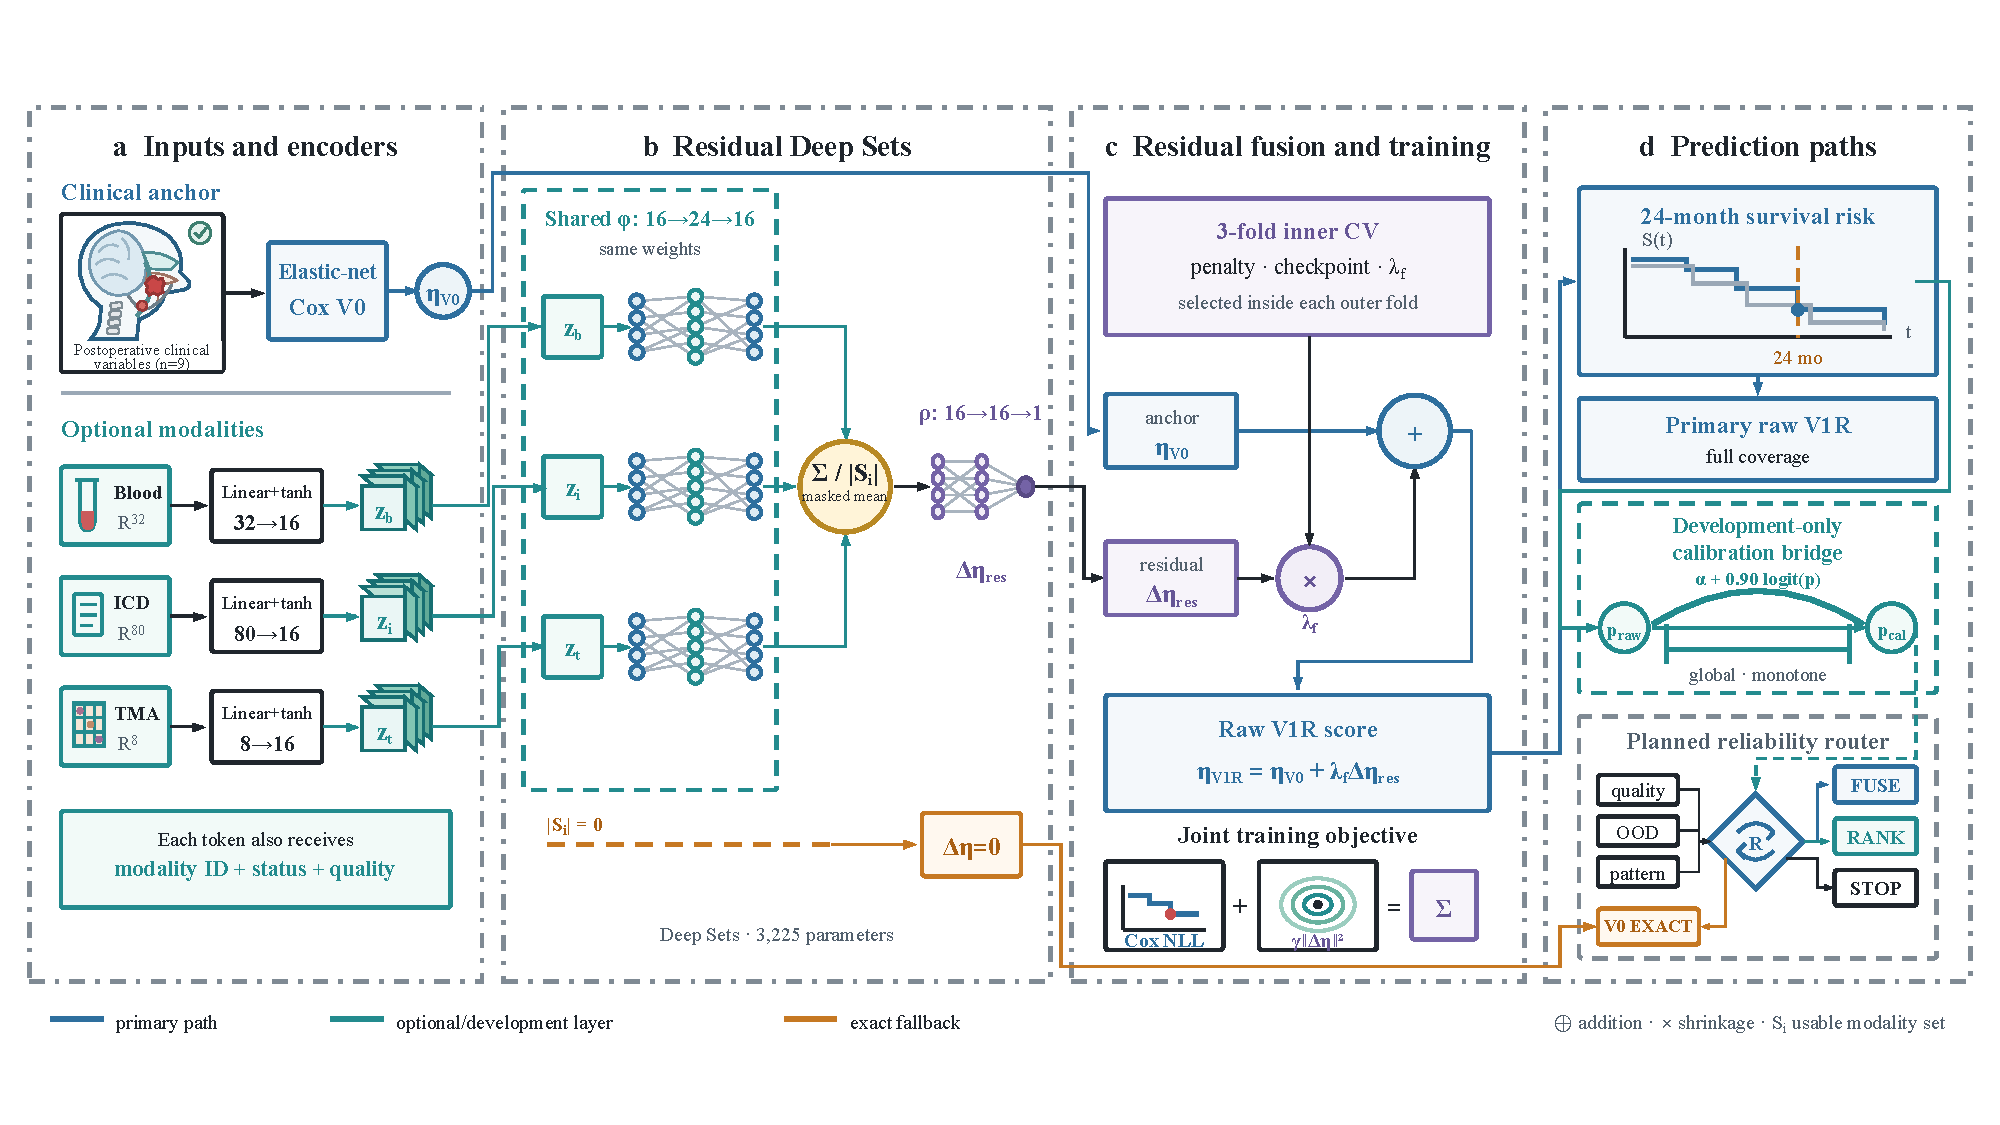
\includegraphics[width=\textwidth]{figures/figure1_pattern_surv_hn_framework.pdf}
\caption{\textbf{Clinically anchored residual fusion architecture for PATTERN-Surv-HN.} \textbf{a}, Postoperative clinical-pathological variables are encoded by CAM. \textbf{b}, Usable blood, ICD and TMA measurements are represented as unordered modality tokens with identity, availability/usability and quality indicators and processed by a shared permutation-invariant Deep Sets residual encoder. \textbf{c}, The residual is shrinkage-controlled and added to CAM to produce raw SCRF; residual penalty, optimization checkpoint and fold-specific scale are selected in inner cross-validation. \textbf{d}, The primary prediction path is raw SCRF with full coverage. If no optional modality is usable, the residual is zero and CAM is returned exactly. The global bridge is development-only; the reliability router is exploratory and not a validated deployment component.}\label{fig:architecture}
\end{figure*}

CAM was an elastic-net Cox proportional-hazards model using age, sex, smoking, primary site, grade, p16, resection, pathological T category and pathological N category \cite{cox1972,breslow1974}. Adjuvant treatment and post-treatment variables were excluded. After training-fold preprocessing,
\begin{equation}
\eta_{\mathrm{CAM},i}=x_{c,i}^{\mathsf T}\hat\beta_c.
\end{equation}
Encoding, imputation, scaling and category handling were confined to the training fold, and a training-fold Breslow baseline hazard converted the linear predictor to 24-month risk.

Each usable optional modality was represented as an unordered token containing measurements, modality identity, usability/status indicators and quality features. A permutation-invariant Deep Sets residual encoder processed the available token set:
\begin{equation}
h_i=\rho\left(\frac{1}{|\mathcal{M}_i|}\sum_{m\in\mathcal{M}_i}\phi(x_{im},q_{im},e_m)\right),\qquad
\Delta\eta_{\mathrm{res},i}=g(h_i).
\end{equation}
The fused score was
\begin{equation}
\eta_{\mathrm{SCRF},i}=\eta_{\mathrm{CAM},i}+\lambda_f\Delta\eta_{\mathrm{res},i}.
\end{equation}
The backbone contained 3,225 parameters. When $\mathcal{M}_i$ was empty, both the residual and fused-score deviation were exactly zero, so the returned prediction equalled CAM. This property made fallback deterministic rather than learned and allowed full-coverage performance to be evaluated without replacing unavailable patients.

\subsection{Nested cross-fitting and optimization}
Development used five outer folds, three inner folds and repetition seeds 17, 29, 43, 71 and 101. For each outer fold $f$, preprocessing, feature handling, model fitting, residual penalty, optimization checkpoint, shrinkage scale and baseline-hazard estimation were confined to training data. Inner cross-validation searched residual penalties $\{0.01,0.1,1.0\}$, checkpoints $\{0,10,25,50\}$ and residual scales $\{0.1,0.2,0.3,0.4,0.5,1.0\}$. No outer-fold outcome information was used to choose these values. Repeated predictions yielded 25 matched CAM/SCRF members (five seeds by five outer folds), allowing both fold-level pairing and seed-level direction summaries.

The formal component ablation reused the same development population, five repetition seeds, outer-fold assignments and endpoint. CAM removed the optional-modality residual pathway. URF retained the identical 3,225-parameter Deep Sets residual architecture but fixed residual scale at 1.0. SCRF additionally allowed the residual scale to be selected inside each inner loop. This staged comparison isolates the contribution of the multimodal branch from the contribution of shrinkage control without changing cohort membership, preprocessing scope or evaluation metrics.

\subsection{Published-method benchmark}
The established-method benchmark compared SCRF with clinical Cox proportional hazards, direct elastic-net Cox, random survival forests, gradient boosting survival analysis, XGBoost-Cox, DeepSurv, single-event DeepHit and an adapted MultiSurv architecture \cite{cox1972,simon2011,ishwaran2008,hothorn2006,chen2016,katzman2018,lee2018,valesilva2021}. The recent-fusion benchmark followed the comparator taxonomies used by two 2026 missing-modality studies and added early feature fusion, late decision fusion, masked attention, low-rank bilinear interaction, missing-aware intermediate fusion and HAF \cite{ruffini2026,zheng2026}. These families complement established multimodal survival designs based on modality dropout, co-attention and pathway-level interaction modelling \cite{cheerla2019,chen2021mcat,jaume2024survpath}. The exact SCRF outer-fold assignments were reused for all methods. Within each outer training fold, numerical imputation, scaling, categorical encoding and missingness/status construction were fitted without held-out rows. Clinical Cox used the clinical-pathological block; all other comparators received clinical, blood, ICD and TMA features, with unusable modality values masked and usability, status and missing-fraction features retained. Every method returned a prediction for every patient.

Classical-model configurations were fixed in the established-method benchmark specification: elastic-net Cox used $\alpha=0.05$ and an equal L1/L2 mixture; random survival forests used 300 trees and a minimum leaf size of 10; gradient boosting used 150 depth-2 learners; and XGBoost-Cox used 200 depth-3 trees with row and column subsampling. DeepSurv and DeepHit were implemented with \texttt{pycox} 0.3.0 and two hidden layers of 64 and 32 units for 160 epochs. DeepHit used 12 discrete intervals with the published likelihood-plus-ranking objective. Adapted MultiSurv used separate 32-dimensional clinical, blood, ICD and TMA encoders, element-wise maximum fusion over usable modalities and a 12-interval conditional-hazard head.

The recent-fusion configuration was frozen before the expanded benchmark run. Early fusion concatenated masked features and availability indicators before a shared head. Late fusion averaged independently supervised modality-specific hazard logits over inputs available to each patient. Masked attention learned a weighted average of available embeddings without latent alignment, whereas bilinear fusion added low-rank pairwise embedding interactions. The Ruffini adaptation trained modality-specific prognostic encoders, froze them and fitted a mask-aware intermediate-fusion head to their concatenated representations. The HAF adaptation used detached prognostic encoders, global pairwise latent alignment and mask-robust gated fusion with a monotonic loss discouraging deterioration when an available modality was added. Because the original studies used CT, whole-slide imaging, molecular data or seven HANCOCK modalities, these rows are explicitly labelled adaptations rather than exact reproductions; a common 12-interval censoring-aware hazard head aligned them with the present time-to-event estimand \cite{gensheimer2019}. Results were summarized as the mean and standard deviation across five complete repeated OOF sets. Both comparator analyses are post-hoc exploratory benchmarks and do not redefine the locked SCRF claim.

\subsection{Development calibration bridge}
For held-out outer fold $f$, raw SCRF risk was transformed by
\begin{align}
x_{\mathrm{raw},i}&=\operatorname{logit}(p_{\mathrm{SCRF},i}),\\
x_{\mathrm{bridge},i}&=\alpha_{\mathrm{logloss},f}+0.90x_{\mathrm{raw},i},\qquad
p_{\mathrm{bridge},i}=\sigma(x_{\mathrm{bridge},i}).
\end{align}
The intercept was fitted by weighted log-loss using only non-held-out development folds. The slope was fixed positive, and no pattern-specific parameters were introduced. Consequently, the bridge was global, strictly monotone and rank-preserving, and it did not alter CAM, raw SCRF, fallback or coverage. The diagnostic population comprised 2,460 repeated out-of-fold rows and 415 evaluable events. Prespecified gates were global Brier change $\le +0.0005$, worst supported-pattern regret $\le +0.005$, improved calibration-in-the-large and slope, preserved ranking and full coverage.

\subsection{Locked confirmation protocol}
Before confirmation outcomes were accessed, the protocol, input manifest, dependency lock and patient-level prediction artifact were frozen. Twenty-five matched members were generated using development-fold fitting only, with no confirmation tuning, bridge, router, refitting, threshold selection or patient removal. Outcomes were read only after prediction sealing. The primary readout was raw SCRF. Aggregate uncertainty used 2,000 patient-level stratified bootstrap replicates (seed 20260825). The locked secondary bridge analysis separately applied the already frozen $\beta=0.90$ transformation with the arithmetic mean development intercept $\alpha=-0.1450338$, using 2,000 event-stratified replicates (seed 20260827); it was labelled a post-unseal readout.

\subsection{Selective routing and extension analyses}
The reliability-aware router first averaged repeated out-of-fold predictions to one row per patient. A five-fold patient-level cross-fitted logistic router selected raw SCRF or CAM using either core value features or reliability-augmented features, including across-repetition standard deviations of CAM risk, SCRF risk and their difference. Fixed thresholds were 0.40, 0.50 and 0.60; 2,000 bootstrap replicates quantified uncertainty.

The RADCURE characterization evaluated adapted clinical/radiomics comparator families C1--C4 on the held-out test split. Transcriptome method replication evaluated residual shrinkage with transcriptome tokens in TCGA-HNSC: 14,417 common genes were represented as within-sample ranks, each training fold retained the 500 most variable genes, and a Linear(500$\rightarrow$32), Tanh, Linear(32$\rightarrow$1) residual head supplied a transcriptome residual. The cross-platform transcriptome characterization fitted one transcriptome SCRF model on the complete TCGA development cohort and applied it without cohort-specific refitting to GSE65858 and GSE41613. Detailed definitions and aggregate outputs are provided in Supplementary Information sections S8--S11.

\subsection{Estimands and statistical analysis}
The paired primary estimand was
\begin{equation}
\Delta\mathrm{Brier}_{24}=\mathrm{Brier}_{24}(\mathrm{SCRF})-\mathrm{Brier}_{24}(\mathrm{CAM}),
\end{equation}
with analogous deltas for Uno C, horizon AUC and Harrell C. Lower Brier and higher discrimination values are better. Calibration-in-the-large is better closer to zero; calibration slope is better closer to one. Pattern safety used
\begin{equation}
\mathcal{R}_{\mathrm{worst}}=\max_{p\in\mathcal{P}_{\mathrm{supported}}}
\{\mathrm{Brier}_{24}(\mathrm{candidate},p)-\mathrm{Brier}_{24}(\mathrm{reference},p)\}.
\end{equation}
IPCW Brier scores, Uno C and time-dependent AUC addressed censoring \cite{graf1999,uno2011}. Bootstrap resampling was performed at patient level, preserving the paired nature of model comparisons. Two-sided 95\% intervals are percentile bootstrap intervals from the prespecified replicate sets.

\subsection{Reproducibility, artifact governance and ethics}
Repetition seeds, split roles, hash identities and aggregate-source paths were recorded for each analysis. The formal development out-of-fold SHA256 was \hashid{E43BB6C0D8E2C7F9C8B22A9C416AD752109B926A8526273D88811458CD73BCE0}; the confirmation protocol SHA256 was \hashid{1E134D30557D1CC153997F6EBB79E99C2E160F85A9F94BF3BBDD81C2C588BDED}; and the sealed prediction artifact SHA256 was \hashid{E5DA83BDB3BB97C3488687C78CCF166FBD03059619DD0690E2767CAF8F393FCF}. Two CAM reruns (internal artifact V0) produced identical out-of-fold hashes. All result figures and tables were generated from aggregate JSON artifacts; no patient-level predictions are included in the manuscript repository.

This analysis used retrospective datasets under their original governance and access conditions; no participants were newly recruited. Dataset-specific review-board approval, consent/waiver language, accessions, versions and secondary-analysis exemptions remain to be reproduced before submission. No patient or public involvement has yet been documented. A large-language-model-assisted coding and writing tool helped organize code, wording and LaTeX; it was not an author and did not independently generate or validate results. Final author verification is required.

\section*{Acknowledgements}
\TBD{Funding, data contributors, collaborators and computing resources.}

\section*{Data availability}
HANCOCK, TCGA-HNSC, GSE65858, GSE41613 and RADCURE are available subject to source conditions \cite{dorrich2025,tcga2015,wichmann2015,lohavanichbutr2013,welch2024}. The repository tracks aggregate metrics, frozen specifications, audits and figure-generation code. Patient-level predictions remain outside version control and will not be redistributed contrary to source terms. \TBD{Add final accession/version table and archival DOI.}

\section*{Code availability}
The configuration-driven \texttt{trust-hn} repository contains model code, frozen contracts, aggregate audits and tests. \TBD{Add public archival release, licence, environment lock and runtime details.}

\section*{Protocol and analysis availability}
The frozen confirmation protocol, analysis specification, aggregate result manifests and artifact hashes are retained with the study materials. Patient-level prediction files remain access-controlled. \TBD{Add the permanent protocol and analysis-plan archive or the process for reasonable-access requests.}

\section*{Author contributions}
\TBD{Complete CRediT roles for all authors.}

\section*{Competing interests}
The authors declare \TBD{no competing interests / specify}.

\section*{Additional information}
\textbf{Supplementary information:} the Supplementary Information provides sections S1--S17, Figs.~S1--S6 and Tables~S1--S10, covering evidence architecture, cohort and leakage procedures, model implementation, component ablation, pattern-level stability, locked confirmation, reliability routing, RADCURE benchmarking, transcriptome method replication, platform transport and published-method diagnostics. The completed TRIPOD+AI checklist and PROBAST+AI assessment will accompany the submission package.\\
\textbf{Correspondence:} \TBD{corresponding author}.\\
\textbf{Provenance and peer review:} \TBD{journal completion}.

% Supplementary Information is intentionally inlined so the complete article
% and supplement are defined and compiled from this single main.tex source.
\clearpage
\section*{Supplementary Information}

This Supplementary Information expands the main-text Methods and Results. It documents the evidence architecture, cohort contracts, model implementation, leakage controls, statistical plan, locked confirmation, routing exploration and extension analyses in RADCURE, TCGA-HNSC and GEO. All numerical summaries are derived from frozen aggregate artifacts; no patient-level predictions are included.

\setcounter{figure}{0}
\setcounter{table}{0}
\renewcommand{\thefigure}{S\arabic{figure}}
\renewcommand{\thetable}{S\arabic{table}}
\renewcommand{\theHfigure}{supp.figure.\arabic{figure}}
\renewcommand{\theHtable}{supp.table.\arabic{table}}
\setlength{\LTcapwidth}{\textwidth}
\renewcommand{\arraystretch}{1.22}

\section*{S1~Evidence architecture and claim map}
The study was organized as a staged evidence pipeline. Repeated nested cross-fitting in the HANCOCK development cohort quantified the incremental value of SCRF over CAM. A monotone calibration bridge was then optimized and evaluated within development folds. Raw SCRF predictions and all analysis dependencies were sealed before confirmation outcomes were accessed. Finally, router, RADCURE, transcriptome and GEO analyses examined selective use, contemporary benchmarking, method transfer and platform transport.

This architecture separates four claims. First, SCRF showed a reproducible development gain, favourable in all five repetition seeds, with complete coverage and pattern-level safety within the prespecified boundary. Second, the HANCOCK confirmation cohort showed favourable point estimates for every principal metric; the bootstrap intervals reflected the moderate event count and supported a consistent directional signal. Third, the development bridge improved calibration summaries, whereas the later bridge readout identified cohort-level probability recalibration as the next step for transportable absolute-risk output. Fourth, router and extension analyses provide design insight and transport evidence complementary to the locked raw-SCRF result.

This separation is a strength of the study. Model development, calibration, confirmation and extension are distinguished by frozen protocols and explicit artifact boundaries. The central finding---controlled incremental multimodal evidence can improve risk ranking while preserving full output availability---can therefore be evaluated alongside calibration, routing and transport considerations without conflating exploratory signals with locked confirmation.

\section*{S2~HANCOCK cohorts, prediction time and endpoint}
HANCOCK was the primary development and confirmation ecosystem. The development analysis included 610 eligible postoperative patients with 173 deaths; the locked confirmation analysis included 152 patients with 40 events. Of 763 source records, one was excluded and 762 eligible postoperative patients remained. The split preserved a separately sealed outcome cohort while retaining sufficient development events for repeated nested cross-fitting.

For patient $i$, $T_i$ denotes event time, $C_i$ censoring time, $Y_i=\min(T_i,C_i)$ observed duration and $\delta_i=I(T_i\le C_i)$ the event indicator. Follow-up began at first treatment and ended at last information; the event was all-cause death. Non-positive durations were excluded. The primary horizon was $t^*=730.5$ days, approximately 24 months. The intended prediction time was immediately after definitive surgery and pathological review, using information available at that point and excluding post-prediction outcome information.

The clinical anchor used age, sex, smoking, primary site, grade, p16, resection, pathological T category and pathological N category. Optional blood, ICD-coded comorbidity and tissue-microarray inputs were admitted only through the residual pathway. This ordering mirrors clinical deployment: the anchor contains routinely available postoperative variables, whereas optional modalities may differ in completeness and preprocessing success.

\section*{S3~Acquisition, usability and quality contract}
For optional modality $m$, the contract distinguished acquisition $a_{im}$, usability $u_{im}$ and an outcome-blind quality vector $q_{im}$. Acquisition indicated that a source record or assay existed. Usability indicated that the frozen preprocessing contract could produce a valid model input. The usable set was
\begin{equation}
\mathcal{M}_i=\{m:u_{im}=1\}.
\end{equation}

Quality summaries included missing fraction, out-of-range counts, assay completeness and distributional distance from training data. Absent and acquired-but-unusable measurements were represented structurally rather than as zero-valued biology. The natural acquisition pattern was the blood--ICD--TMA usability tuple. Pattern counts and quality distributions were computed without outcomes. For development safety analyses, a supported pattern required at least 30 patients and 10 events; rarer patterns were descriptive and did not receive pattern-specific tuning.

Of 762 eligible patients, 693 blood, 712 ICD and 736 tissue-microarray records were acquired, whereas 683, 712 and 736, respectively, were usable. Thus, ten acquired blood records failed the usability contract. Complete blood and TMA records numbered 604 and 639; 79 blood and 97 TMA records were partially usable. This contract preserves the distinction between absence, partial usability and acquired-but-unusable evidence.

The clinical-pathological anchor was fixed to age at diagnosis, sex, smoking status, primary tumour site, grade, p16 association, resection status, pathological T category and pathological N category. Pathology belonged to the postoperative anchor rather than being treated as an optional token. Adjuvant treatment, recurrence, progression, metastasis recorded after the prediction time and outcome-derived variables were prohibited predictors. Optional blocks remained separate at the data boundary; they were not concatenated into a complete-case matrix before availability and usability had been assigned.

The blood block used a fixed panel of 16 haematology measurements from the prespecified pre-treatment window. A missing blood row denoted non-acquisition, whereas a present row with invalid or entirely missing measurements could be acquired but unusable. Partially observed usable rows retained within-block missingness for fold-bound imputation and explicit missingness indicators. TMA followed the same structural rule: absence of a row represented modality absence; missing values within an existing row represented within-modality incompleteness. This distinction prevented biological zeros from being substituted for unavailable assays.

The locally available ICD block consisted of 40 pre-extracted code groups. The underlying vocabulary had been generated with a corpus-level minimum document frequency of three, and the raw text source was not available for reconstruction. ICD was therefore marked as having conditional provenance. It was retained in the frozen evidence contract, but this limitation is disclosed because a fully fold-pure vocabulary sensitivity analysis would be preferable in a future release.

Separate fold-bound preprocessors handled the clinical mixed-type block and the three numeric optional blocks. Training-fold medians, scaling parameters, categorical levels and one-hot mappings were estimated only from explicitly allowed fit identifiers. New categories at transform time mapped to an unknown level. The preprocessing interface rejected held-out identifiers during fitting and returned missingness indicators alongside transformed values. These checks made leakage control executable rather than dependent only on analyst convention.

\section*{S4~Clinical anchor and residual network}
CAM was an elastic-net Cox proportional-hazards model \cite{cox1972,breslow1974}. After training-fold preprocessing,
\begin{equation}
\eta_{\mathrm{CAM},i}=x_{c,i}^{\mathsf T}\hat\beta_c.
\end{equation}
Encoding, imputation, scaling and category handling were confined to the corresponding training fold. A training-fold Breslow baseline-hazard estimator converted the linear predictor to 24-month mortality risk.

SCRF was a clinically anchored residual Deep Sets Cox backbone with 3,225 parameters. Each usable modality was represented as an unordered token containing its measurements, learned representation, modality identity, usability status and quality indicators:
\begin{equation}
h_i=\rho\left(\frac{1}{|\mathcal{M}_i|}\sum_{m\in\mathcal{M}_i}\phi(x_{im},q_{im},e_m)\right),\qquad
\Delta\eta_{\mathrm{res},i}=g(h_i).
\end{equation}
The fused score was
\begin{equation}
\eta_{\mathrm{SCRF},i}=\eta_{\mathrm{CAM},i}+\lambda_f\Delta\eta_{\mathrm{res},i}.
\end{equation}
The token form makes the input set permutation invariant, while the masked mean allows any non-empty usable subset to be processed. When $\mathcal{M}_i$ is empty, the residual and fused-score deviations are exactly zero, so SCRF returns CAM deterministically.

\section*{S5~Nested cross-fitting, optimization and leakage control}
Repeated nested cross-fitting used five outer folds, three inner folds and repetition seeds 17, 29, 43, 71 and 101. Preprocessing, feature selection where applicable, model fitting, shrinkage selection and baseline-hazard estimation were confined to training folds. For each outer fold $f$, inner cross-validation searched residual penalties $\{0.01,0.1,1.0\}$, optimization checkpoints $\{0,10,25,50\}$ and residual scales $\{0.1,0.2,0.3,0.4,0.5,1.0\}$.

This design yields 25 matched CAM/SCRF members (five seeds by five outer folds) and supports paired fold-level and seed-level summaries. Outer-fold outcomes were not used for hyperparameter selection. Repeated out-of-fold rows provided the development performance estimates and the calibration-bridge diagnostic, while seed-level paired differences assessed reproducibility. No confirmation outcomes entered development tuning.

The SCRF stage was a transparently result-informed rescue of the original unshrunk URF analysis. The original U2 decision, retained internally as \texttt{V1\_DOES\_NOT\_EARN\_COMPLEXITY}, remains unchanged. Prediction-space sensitivity analysis indicated that the unscaled residual was too aggressive; scales near 0.2--0.4 reduced pattern regret and calibration-slope deterioration while retaining a small, seed-stable discrimination signal. SCRF therefore added residual scale to the inner-loop search and was labelled post-hoc exploratory rather than retrospectively reclassifying the original URF result.

The frozen SCRF selection objective minimized mean inner-fold IPCW Brier score at 730.5 days, with mean inner-fold Uno C as the secondary criterion. Deterministic ties favoured the larger residual penalty, then the smaller residual scale, then fewer optimization steps. Architecture search and broad hyperparameter sweeps were prohibited. The implementation used deterministic PyTorch computation on CPU in float64, Adam optimization with learning rate 0.003, weight decay 0.0001 and gradient clipping at norm 5.0. The loss combined mean negative Breslow partial likelihood with an L2 penalty on the residual score.

After the inner-loop candidate was selected, the corresponding outer-training fold was refitted and its Breslow baseline hazard was estimated after residual scaling using training outcomes only. Each patient was predicted exactly once per repetition. Patient-level out-of-fold predictions were stored outside tracked manuscript artifacts; only aggregate audits and frozen specifications were committed. The rescue gate retained the original safety thresholds and could authorize only a development signal, not confirmatory superiority or external validation.

\section*{S6~Global calibration bridge}
The U5R7 bridge was frozen as \texttt{beta\_0.900\_logloss}. For raw SCRF 24-month risk $p_{\mathrm{SCRF}}$ in held-out outer fold $f$,
\begin{align}
x_{\mathrm{raw},i}&=\operatorname{logit}(p_{\mathrm{SCRF},i}),\\
x_{\mathrm{bridge},i}&=\alpha_{\mathrm{logloss},f}+0.90x_{\mathrm{raw},i},\qquad
p_{\mathrm{bridge},i}=\sigma(x_{\mathrm{bridge},i}).
\end{align}
The intercept was fitted by weighted log-loss using only non-held-out development folds. The bridge was global and pattern-agnostic, with a fixed positive slope. It was therefore strictly monotone, preserved ranking, retained 100\% coverage and did not alter the exact CAM fallback.

The diagnostic population contained 2,460 repeated out-of-fold rows and 415 evaluable events. Gates were global Brier change $\le +0.0005$, worst supported-pattern regret $\le +0.005$, improved calibration-in-the-large and calibration slope, ranking preservation and full coverage. Confirmation outcomes were not used for fitting or tuning.

U5R7 followed a sequence of development-only bridge explorations and froze the candidate identifier \texttt{beta\_0.900\_logloss} before its diagnostic readout. The positive slope was not estimated separately by pattern, and the intercept was fitted anew within each non-held-out development partition. Thus, the bridge could move the absolute probability scale without changing within-fold ordering. It also left the raw SCRF score, CAM, acquisition rules and empty-set fallback untouched.

The bridge diagnostic is not numerically interchangeable with the primary development table. It contains repeated evaluable out-of-fold rows and addresses whether a global monotone transformation improves absolute-risk calibration; the primary table compares CAM and raw SCRF as prediction models. The small positive Brier change was retained in the report rather than hidden. U5R7 passed its prespecified development-safe gates, but the decision authorized only a development calibration candidate. Raw SCRF remained the primary prediction path and the only fused model carried into the locked confirmation comparison.

\section*{S7~Locked confirmation and secondary bridge protocol}
The confirmation protocol, input manifest, dependency lock and prediction artifact were frozen before confirmation outcomes were unsealed. Twenty-five matched CAM/SCRF members were generated using five seeds and five outer folds, with development-fold fitting only and no confirmation tuning, bridge, router, refitting or selective patient removal. Outcomes were read after prediction sealing.

Aggregate uncertainty used 2,000 patient-level stratified bootstrap replicates (seed 20260825). The primary confirmation readout was raw SCRF. U5R8 separately reused the frozen $\beta=0.90$ bridge with the arithmetic mean development intercept $\alpha=-0.1450338$, using 2,000 event-stratified replicates (seed 20260827). Because U5R8 occurred after raw-outcome unsealing, it is reported as a locked secondary post-unseal validation and is interpreted as evidence about probability-scale transport rather than ranking.

The locking sequence separated prediction generation from outcome evaluation. The sealed input manifest identified the eligible confirmation records and the exact source variables consumed by CAM and SCRF. The dependency receipt fixed the execution environment, and the prediction receipt recorded the patient-level artifact before the event file was joined. Aggregate metrics were then computed from the sealed predictions. The confirmation cohort therefore supplied no information for preprocessing, hyperparameter choice, residual shrinkage, baseline-hazard estimation, threshold selection or model refitting.

The 25 members were kept matched between CAM and SCRF so that every paired contrast compared predictions obtained under the same repetition and outer-fold training role. Coverage was evaluated before performance summaries and remained 100\% for both models. Bootstrap sampling operated on patients rather than the 25 repeated prediction rows; this preserved within-patient dependence and prevented artificial precision from treating repeated predictions as independent observations. The bridge was excluded from the primary confirmation estimand because it had been developed as a separate calibration layer. Its later reuse in U5R8 did not modify the locked raw-SCRF result.

\section*{S8~Reliability-aware router design}
The U6R1 router evaluated whether patient-level reliability information could choose between raw SCRF and CAM. Repeated out-of-fold predictions were first averaged to one row per patient. A five-fold patient-level cross-fitted logistic router used either core value features or reliability-augmented features. Reliability features included across-repetition standard deviations of CAM risk, SCRF risk and their difference. Thresholds 0.40, 0.50 and 0.60 were fixed before readout.

Router performance was compared with both CAM and direct raw SCRF. The primary probabilistic readout was IPCW Brier score at 24 months. FUSE rate, delta versus CAM, delta versus raw SCRF and rank concordance with raw SCRF summarized behaviour. Bootstrap resampling used 2,000 replicates. This matched-coverage design tests whether stability information adds routing value without rewarding patient exclusion.

The router used fixed logistic regularization $C=0.5$. A FUSE decision returned raw SCRF; a FALLBACK decision returned CAM. It did not abstain, remove patients or create a third risk model, so every policy retained 100\% prediction availability. Core features summarized the cross-fitted value contrast between the two candidate predictions. The reliability-augmented version added the across-repetition standard deviation of CAM risk, SCRF risk and their patient-level difference, thereby asking whether a stable apparent gain should be treated differently from an equally large but unstable gain.

The thresholds were intentionally reported as a panel rather than selected after observing the final metric. At lower thresholds, more patients followed SCRF; at higher thresholds, the router required stronger evidence before fusing. Rank concordance with raw SCRF was included because switching individual patients back to CAM can change global ordering even when Brier score improves. Direct raw SCRF remained the strongest point-estimate policy, and the best router's bootstrap interval crossed zero. U6R1 therefore supports reliability-aware selection as a research question, not as a validated deployment component or a replacement for the full-coverage primary path.

\section*{S9~RADCURE comparator characterization design}
U7R2 evaluated adapted clinical/radiomics comparator families C1--C4 in the RADCURE held-out test split. The analysis included 626 patients and 110 events. The purpose was to benchmark a contemporary clinical/tumour-volume modelling task and to characterize discrimination, probabilistic error and calibration in a held-out imaging-rich cohort. Comparators were adapted to the RADCURE evidence contract; the current HANCOCK blood--ICD--TMA SCRF artifact was not evaluated because the frozen optional-modality inputs and preprocessing contract did not map directly onto RADCURE.

The characterization reports IPCW Brier score, Uno C at 24 months, time-dependent AUC, Harrell C, calibration-in-the-large and calibration slope. This analysis provides a strong contextual benchmark and shows the practical value of combining clinical predictors with tumour-volume information. It is interpreted as comparator characterization rather than current-SCRF external validation.

Before U7R2, the external-cohort intake procedure was frozen for a possible formal current-SCRF confirmation. A qualifying cohort had to reproduce the required postoperative prediction time, clinical-pathological anchor variables, blood, ICD and TMA evidence definitions, endpoint, follow-up horizon and outcome-untouched status. The available inventory contained no cohort satisfying all of these conditions. RADCURE was therefore chosen only for the narrower task that its clinical and radiomic variables could support.

The held-out RADCURE test split was not used to tune any HANCOCK model, calibration bridge, router threshold or safety gate. Conversely, its comparator families were adapted to the RADCURE data contract and are not numerical surrogates for the current SCRF artifact. RADCURE outcomes had also been consumed in earlier work, precluding an outcome-untouched confirmation label. These constraints are why the analysis is described as external characterization: it tests the plausibility of combining clinical information with an image-derived tumour-volume representation, but does not establish transportability of blood--ICD--TMA residual fusion.

\section*{S10~TCGA transcriptome residual replication design}
U8 tested transfer of the residual-shrinkage principle from sparse HANCOCK optional modalities to a dense transcriptome modality. The analysis included 519 TCGA-HNSC patients and 221 events. The clinical anchor used age, sex, site, stage, HPV status, treatment and smoking. The transcriptome contained 14,417 common genes represented as within-sample ranks; each training fold retained the 500 most variable genes.

The residual head was Linear(500$\rightarrow$32), Tanh, Linear(32$\rightarrow$1), and the fused score was
\begin{equation}
\eta_{\mathrm{tSCRF},i}=\eta_{\mathrm{CAM},i}+\lambda_f\Delta\eta_{\mathrm{transcriptome},i}.
\end{equation}
All selection steps were confined to training folds. The completed run produced 2,595 out-of-fold rows with complete coverage and an exact fallback error of zero. We refer to this analogue as transcriptome SCRF (tSCRF; internal artifact T1R). Because TCGA outcomes had already been consumed during analysis development, this experiment is labelled post-hoc method replication: it tests whether the architectural principle transfers to transcriptome data, rather than providing a pristine external validation of SCRF.

The replication used five outer folds, three inner folds and the same repetition seeds 17, 29, 43, 71 and 101. Within every outer-training partition, clinical preprocessing, elastic-net anchor selection, the 500-gene variance filter, residual fitting, residual-penalty choice, optimization checkpoint, shrinkage scale and Breslow baseline hazard were estimated without the held-out fold. The transcriptome residual head contained 16,065 trainable parameters, below the frozen 50,000-parameter ceiling. The acquisition-pattern safety check collapsed to the single transcriptome-present pattern, while the score construction retained exact zero-residual fallback as a structural test.

The frozen exploratory gate required complete coverage, structural fallback safety, bounded Brier deterioration, bounded calibration deterioration and at least one reproducible incremental-value path. Observed worst supported-pattern Brier regret was $+0.002714$ against a $+0.020$ ceiling. Mean absolute calibration-in-the-large deterioration was $+0.049232$ against a $+0.100$ ceiling, and mean absolute calibration-slope-error deterioration was $-0.084226$ against a $+0.150$ ceiling. Both probability-error and discrimination paths met their seed-stability requirements, so the frozen gate returned \texttt{T1R\_EARNS\_COMPLEXITY}.

That gate result has a deliberately limited meaning. It authorizes the statement that the residual-shrinkage principle showed internal value in a dense transcriptome setting; it does not establish current-SCRF external validity, pristine confirmation, clinical utility or deployment readiness. It also does not replace the HANCOCK backbone or alter the locked raw-SCRF confirmation. Patient-level TCGA predictions remain outside the manuscript repository, and the publication table is generated from the aggregate development audit.

\section*{S11~GEO cross-platform transfer design}
U8E applied a single full-development tSCRF fit to GSE65858 and GSE41613 without cohort-specific refitting, tuning or threshold selection. GSE65858 contributed 244 patients and 78 events; GSE41613 contributed 97 patients and 51 events. Before application, inner cross-validation selected an elastic-net anchor with alpha 0.05 and L1 ratio 0.1, residual penalty 1.0, optimization checkpoint 10 and residual scale 1.0.

Within-sample rank representation was retained as the transcriptome input representation. The analysis reports paired Brier, Harrell C, Uno C, time-dependent AUC, calibration-in-the-large and calibration-slope changes. The design emphasizes method transfer and cross-platform signal retention. Calibration slopes above one indicate compressed predicted-risk dispersion, making cohort-level recalibration the natural next step before prospective absolute-risk reporting.

The full-development TCGA fit contained the same 16,065-parameter residual head used during cross-fitting. Development-only inner cross-validation selected elastic-net $\alpha=0.05$, L1 ratio 0.1, residual penalty 1.0, optimization checkpoint 10 and residual scale 1.0 before either GEO cohort was evaluated. The resulting feature-selection and model parameters were carried forward as one frozen package. No GEO-specific gene selection, refitting, hyperparameter search, decision threshold or outcome-dependent cohort selection was performed, and coverage was complete in both cohorts.

GSE65858 provided a conventional test of whether the transcriptome residual preserved ordering beyond a varying clinical anchor. GSE41613 provided a complementary edge case: the applied anchor had no cross-patient variation, so its discrimination was 0.5 and any recovered ordering arose from the transported transcriptome component. In both cohorts, Brier score and all discrimination summaries changed favourably, while calibration behaviour remained cohort dependent. This combination of results distinguishes transport of relative ordering from transport of absolute probability scale.

Because both GEO outcome sets had contributed to earlier Phase 6 analyses, the application is explicitly post-hoc characterization. Concordant directions across the two cohorts strengthen the plausibility of the transcriptome residual signal, but they are not treated as formal external validation. The appropriate next experiment is to seal predictions in a newly identified outcome-untouched cohort, prespecify any cohort-level recalibration, and evaluate both discrimination and calibration without reusing these GEO outcomes for tuning.

\section*{S12~Implementation and statistical plan}
Paired development and confirmation estimands were
\begin{equation}
\Delta\mathrm{Brier}_{24}=\mathrm{Brier}_{24}(\mathrm{SCRF})-\mathrm{Brier}_{24}(\mathrm{CAM})
\end{equation}
and analogous discrimination deltas. Lower Brier and higher discrimination values are better. Calibration-in-the-large is better closer to zero; calibration slope is better closer to one. Pattern safety used
\begin{equation}
\mathcal{R}_{\mathrm{worst}}=\max_{p\in\mathcal{P}_{\mathrm{supported}}}
\{\mathrm{Brier}_{24}(\mathrm{candidate},p)-\mathrm{Brier}_{24}(\mathrm{reference},p)\},
\end{equation}
where supported patterns required at least 30 patients and 10 events.

IPCW Brier scores, Uno concordance and horizon AUC addressed censoring \cite{graf1999,uno2011}. Two-sided 95\% percentile intervals used prespecified patient-level stratified bootstrap replicate sets. Patients, rather than repeated prediction rows, were resampled for confirmation intervals. Development summaries reported both aggregate means and the number of repetition seeds with a favourable direction. No multiplicity adjustment was applied to exploratory extension readouts; their role is supportive characterization.

The primary horizon was 730.5 days. IPCW weights were estimated within the relevant analysis population, and paired comparisons used the same eligible patients and horizon for both candidate predictions. Uno concordance summarized censoring-adjusted ranking through the horizon; time-dependent AUC summarized case--control separation at the horizon; Harrell concordance was retained as a familiar global ranking measure. IPCW Brier score combined discrimination and calibration as a proper probabilistic loss. Calibration-in-the-large compared average predicted and observed risk on the fitted probability scale, while the calibration slope assessed dispersion.

For natural evidence-pattern analyses, a pattern entered the supported set only when at least 30 patients and 10 events were available. This threshold prevented small cells from becoming independently tuned strata. Rare patterns remained visible in counts and descriptive outputs, but they were not used to justify pattern-specific transport claims. Full-coverage performance always retained patients with no usable optional modality, whose deterministic CAM fallback made the deployment estimand different from a complete-case analysis.

Development cross-fitting produced repeated predictions for stability assessment, but uncertainty calculations respected the patient as the sampling unit. Confirmation intervals were computed from 2,000 patient-level stratified replicates. Router intervals likewise used 2,000 patient bootstrap replicates after repeated predictions had first been aggregated to one row per patient. Extension analyses report prespecified aggregate and seed-direction summaries without multiplicity-adjusted inferential claims. This hierarchy keeps the locked confirmation, development diagnostics and post-hoc characterizations statistically distinct.

\section*{S13~Supporting development and calibration evidence}
SCRF improved every aggregate discrimination measure and the mean 24-month IPCW Brier score in HANCOCK development (Table~\ref{tab:supptable1}). The mean Uno C gain was $+0.021303$ and was favourable in all five seeds. Coverage remained 100\%, the empty-set fallback error was zero, and the worst supported-pattern Brier regret was $+0.009848$, below the $+0.020$ safety boundary.

The U5R7 bridge moved calibration-in-the-large from $+0.011680$ to $-0.003796$ and calibration slope from 0.825887 to 0.881552 (Table~\ref{tab:supptable2}). Ranking and coverage were preserved. The global Brier change was $+0.000147$, within the $+0.0005$ gate, and worst supported-pattern regret was $+0.004176$, below the $+0.005$ gate. Thus, the development bridge improved the probability scale without changing patient ordering or availability.

\begingroup
\scriptsize
\setlength{\tabcolsep}{2pt}
\begin{longtable}{>{\raggedright\arraybackslash}p{0.26\textwidth}rrr>{\raggedright\arraybackslash}p{0.27\textwidth}}
\caption{Development performance of shrinkage-controlled residual fusion}\label{tab:supptable1}\\
\toprule
Metric & CAM & SCRF & Difference & Interpretation\\
\midrule
\endfirsthead
\multicolumn{5}{l}{\itshape Table S1 continued from previous page}\\
\toprule
Metric & CAM & SCRF & Difference & Interpretation\\
\midrule
\endhead
\bottomrule
\endlastfoot
IPCW Brier at 24 months & 0.124745 & 0.124338 & $-0.000407$ & Lower probabilistic error\\
Uno C at 24 months & 0.644239 & 0.665542 & $+0.021303$ & Improved discrimination\\
Time-dependent AUC at 24 months & 0.662022 & 0.682511 & $+0.020488$ & Improved horizon ranking\\
Harrell C & 0.623021 & 0.633710 & $+0.010690$ & Improved overall ranking\\
Coverage & 100\% & 100\% & 0 & Full output availability\\
Empty-set fallback error & 0 & 0 & 0 & Exact clinical fallback\\
Worst supported-pattern Brier regret & Reference & $+0.009848$ & $+0.009848$ & Below $+0.020$ boundary\\
Seeds with improved Uno C & -- & 5/5 & -- & Consistent direction\\
\end{longtable}
\endgroup

The staged ablation (Table~\ref{tab:ablation}) shows why residual shrinkage is part of the proposed mechanism rather than a cosmetic tuning choice. Adding the unshrunk residual pathway alone did not improve the joint discrimination--probability-error profile: its small Uno C gain accompanied worse Brier score and AUC. Inner-selected shrinkage converted the same residual architecture into a seed-stable discrimination gain while recovering the Brier score. All three stages retained the identical full-coverage population; both residual models preserved exact clinical fallback when the optional evidence set was empty.

\begingroup
\footnotesize
\setlength{\tabcolsep}{3pt}
\begin{longtable}{>{\raggedright\arraybackslash}p{0.29\textwidth}rrrr}
\caption{Component ablation of the clinical anchor, residual pathway and shrinkage control}\label{tab:ablation}\\
\toprule
Model stage & IPCW Brier$_{24}$ & Uno C$_{24}$ & AUC$_{24}$ & Harrell C\\
\midrule
\endfirsthead
\multicolumn{5}{l}{\itshape Table S2 continued from previous page}\\
\toprule
Model stage & IPCW Brier$_{24}$ & Uno C$_{24}$ & AUC$_{24}$ & Harrell C\\
\midrule
\endhead
\bottomrule
\endlastfoot
Clinical anchor model (CAM) & 0.124745 & 0.644239 & 0.662022 & 0.623021\\
Unshrunk residual fusion (URF) & 0.126546 & 0.646355 & 0.658904 & 0.627593\\
Shrinkage-controlled residual fusion (SCRF) & \textbf{0.124338} & \textbf{0.665542} & \textbf{0.682511} & \textbf{0.633710}\\
\addlinespace[3pt]
URF minus CAM & $+0.001801$ & $+0.002116$ & $-0.003118$ & $+0.004572$\\
SCRF minus CAM & $-0.000407$ & $+0.021303$ & $+0.020488$ & $+0.010690$\\
\end{longtable}
\endgroup

\begingroup
\scriptsize
\setlength{\tabcolsep}{2pt}
\begin{longtable}{>{\raggedright\arraybackslash}p{0.24\textwidth}rrr>{\raggedright\arraybackslash}p{0.29\textwidth}}
\caption{U5R7 development calibration bridge}\label{tab:supptable2}\\
\toprule
Metric & Raw SCRF & U5R7 bridge & Change & Interpretation\\
\midrule
\endfirsthead
\multicolumn{5}{l}{\itshape Table S3 continued from previous page}\\
\toprule
Metric & Raw SCRF & U5R7 bridge & Change & Interpretation\\
\midrule
\endhead
\bottomrule
\endlastfoot
IPCW Brier at 24 months & 0.126637 & 0.126784 & $+0.000147$ & Within $+0.0005$ gate\\
Calibration-in-the-large & $+0.011680$ & $-0.003796$ & $-0.015477$ & Absolute error improved by 0.007884\\
Calibration slope & 0.825887 & 0.881552 & $+0.055665$ & Absolute error improved by 0.055665\\
Worst supported-pattern Brier regret & Reference & $+0.004176$ & $+0.004176$ & Below $+0.005$ gate\\
Coverage & 100\% & 100\% & 0 & Preserved\\
Ranking & Reference & Preserved & -- & All held-out folds\\
\end{longtable}
\endgroup

\section*{S14~Locked confirmation and routing readouts}
In the 152-patient, 40-event outcome-sealed cohort, raw SCRF showed favourable point estimates for discrimination, Brier score and calibration summaries (Table~\ref{tab:supptable3}). Patient-level stratified bootstrap with 2,000 replicates gave a mean delta Uno C of $+0.021654$ (95\% interval $-0.025965$ to $+0.070816$) and a mean delta IPCW Brier of $-0.005222$ (95\% interval $-0.012843$ to $+0.002171$). The direction was favourable across the principal readouts, with intervals reflecting the moderate event count.

The secondary U5R8 bridge readout preserved ranking and coverage but changed IPCW Brier from 0.134697 to 0.135782, calibration-in-the-large from $+0.156751$ to $+0.160944$ and calibration slope from 1.510335 to 1.678150. This result identifies cohort-level probability recalibration as the key next step for transportable absolute-risk output.

\begingroup
\scriptsize
\setlength{\tabcolsep}{2pt}
\begin{longtable}{>{\raggedright\arraybackslash}p{0.25\textwidth}rrr>{\raggedright\arraybackslash}p{0.28\textwidth}}
\caption{Locked raw-SCRF confirmation}\label{tab:supptable3}\\
\toprule
Metric at 24 months & CAM & Raw SCRF & Difference & Interpretation\\
\midrule
\endfirsthead
\multicolumn{5}{l}{\itshape Table S4 continued from previous page}\\
\toprule
Metric at 24 months & CAM & Raw SCRF & Difference & Interpretation\\
\midrule
\endhead
\bottomrule
\endlastfoot
Uno C & 0.782579 & 0.804242 & $+0.021664$ & Favourable point estimate\\
IPCW Brier & 0.136412 & 0.131246 & $-0.005166$ & Favourable point estimate\\
Time-dependent AUC & 0.801094 & 0.813637 & $+0.012543$ & Favourable point estimate\\
Harrell C & 0.733253 & 0.752842 & $+0.019589$ & Favourable point estimate\\
Calibration-in-the-large & 0.211270 & 0.116482 & $-0.094788$ & Closer to zero\\
Calibration slope & 1.945126 & 1.501223 & $-0.443903$ & Closer to one\\
Coverage & 100\% & 100\% & 0 & Preserved\\
\end{longtable}
\endgroup

Every router improved on CAM at the point estimate, while direct raw SCRF remained the strongest overall policy (Table~\ref{tab:supptable4} and Fig.~\ref{fig:supp_router}). The best router used reliability features at threshold 0.60: delta Brier versus CAM was $-0.000506$, and its bootstrap interval was approximately $-0.00162$ to $+0.00076$. These results show that repetition-level stability contains useful routing information and support further development of selective prediction at matched coverage.

\begingroup
\scriptsize
\setlength{\tabcolsep}{1.5pt}
\begin{longtable}{>{\raggedright\arraybackslash}p{0.23\textwidth}rrrrr}
\caption{Development-only router policies}\label{tab:supptable4}\\
\toprule
Policy & FUSE rate & Brier$_{24}$ & $\Delta$ vs CAM & $\Delta$ vs raw SCRF & Rank concordance\\
\midrule
\endfirsthead
\multicolumn{6}{l}{\itshape Table S5 continued from previous page}\\
\toprule
Policy & FUSE rate & Brier$_{24}$ & $\Delta$ vs CAM & $\Delta$ vs raw SCRF & Rank concordance\\
\midrule
\endhead
\bottomrule
\endlastfoot
CAM & 0.0\% & 0.123927 & 0 & $+0.001162$ & 0.867\\
Raw SCRF & 100.0\% & 0.122765 & $-0.001162$ & 0 & 1.000\\
Core router, $q\ge0.40$ & 66.1\% & 0.123545 & $-0.000382$ & $+0.000780$ & 0.945\\
Core router, $q\ge0.50$ & 54.1\% & 0.123511 & $-0.000416$ & $+0.000746$ & 0.939\\
Core router, $q\ge0.60$ & 40.3\% & 0.123585 & $-0.000341$ & $+0.000821$ & 0.928\\
Reliability router, $q\ge0.40$ & 67.0\% & 0.123648 & $-0.000279$ & $+0.000883$ & 0.946\\
Reliability router, $q\ge0.50$ & 54.8\% & 0.123508 & $-0.000419$ & $+0.000743$ & 0.938\\
Reliability router, $q\ge0.60$ & 42.6\% & 0.123421 & $-0.000506$ & $+0.000657$ & 0.929\\
\end{longtable}
\endgroup

\begin{figure*}[t]
\centering
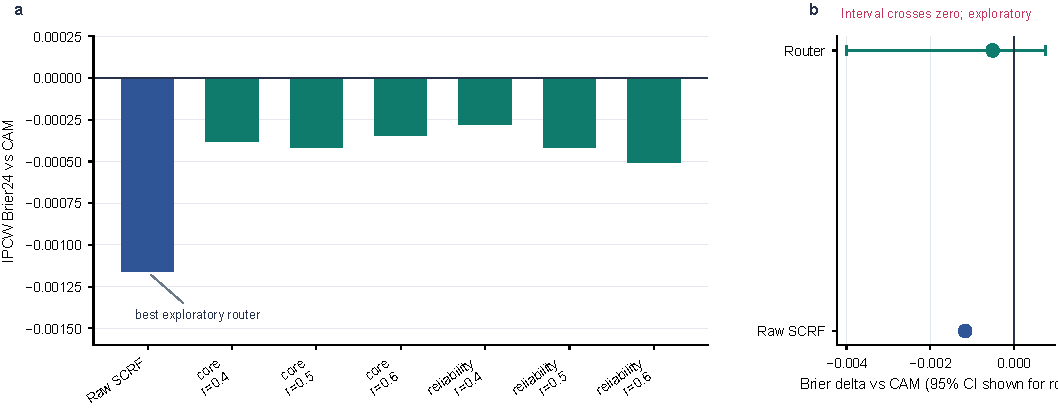
\includegraphics[width=\textwidth]{figures/extended_data_figure1_router_exploration.pdf}
\caption{\textbf{Exploratory patient-level reliability router.} \textbf{a}, IPCW Brier differences versus CAM for raw SCRF and router policies. \textbf{b}, Best router point estimate with bootstrap interval. Reliability features improve routing relative to the core router and CAM, while direct raw SCRF remains the strongest full-coverage policy.}\label{fig:supp_router}
\end{figure*}

\clearpage
\section*{S15~Extension readouts: RADCURE, TCGA and GEO}
The RADCURE held-out analysis characterized adapted clinical/radiomics comparator families in 626 patients with 110 events. The strongest comparator, C2, achieved Uno C 0.806744, 24-month AUC 0.818182 and IPCW Brier 0.090683 (Table~\ref{tab:supptable5} and Fig.~\ref{fig:supp_radcure}). This analysis provides a strong contemporary benchmark for the multimodal prognostic task and highlights the value of combining clinical and tumour-volume information.

\begingroup
\scriptsize
\setlength{\tabcolsep}{3pt}
\begin{longtable}{lrrrrrr}
\caption{RADCURE held-out comparator characterization}\label{tab:supptable5}\\
\toprule
Comparator & Brier$_{24}$ & Uno C & AUC$_{24}$ & Harrell C & CITL & Calibration slope\\
\midrule
\endfirsthead
\multicolumn{7}{l}{\itshape Table S6 continued from previous page}\\
\toprule
Comparator & Brier$_{24}$ & Uno C & AUC$_{24}$ & Harrell C & CITL & Calibration slope\\
\midrule
\endhead
\bottomrule
\endlastfoot
C1 & 0.095801 & 0.806595 & 0.819376 & 0.795924 & $-0.097110$ & 1.950857\\
C2 & 0.090683 & 0.806744 & 0.818182 & 0.797862 & $-0.044444$ & 1.139466\\
C3 & 0.098469 & 0.771260 & 0.780742 & 0.761632 & $-0.099603$ & 1.268349\\
C4 & 0.097403 & 0.779243 & 0.787882 & 0.768812 & $-0.074520$ & 1.471544\\
\end{longtable}
\endgroup

\begin{figure*}[t]
\centering
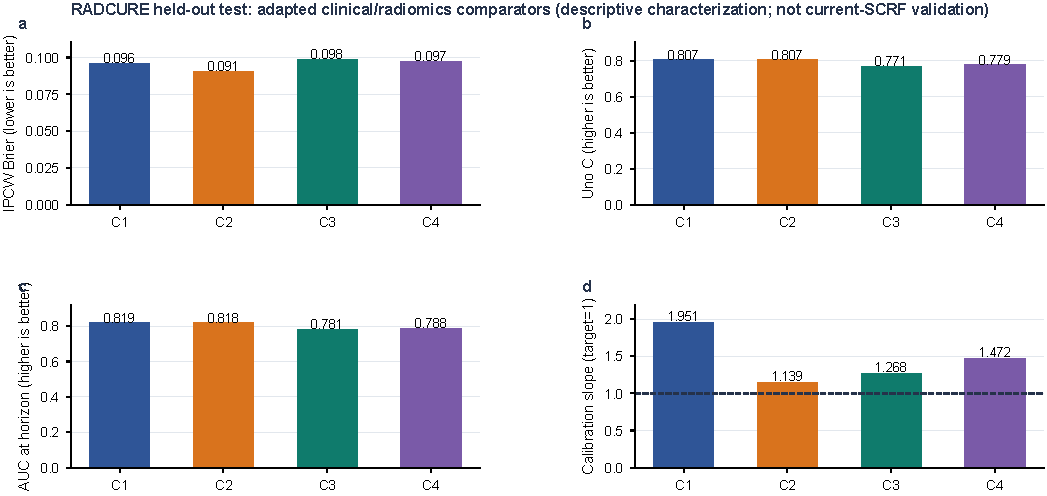
\includegraphics[width=\textwidth]{figures/extended_data_figure2_radcure_characterization.pdf}
\caption{\textbf{RADCURE characterization of adapted clinical/radiomics comparators.} \textbf{a--d}, IPCW Brier, Uno C, horizon AUC and calibration slope for C1--C4 in the held-out test split. C2 provides a strong benchmark by combining clinical predictors with tumour-volume information.}\label{fig:supp_radcure}
\end{figure*}

tSCRF improved every discrimination measure and the mean Brier score in TCGA-HNSC (Table~\ref{tab:supptable6}); discrimination improved in all five seeds (Table~\ref{tab:supptable7} and Fig.~\ref{fig:supp_t1r}). The frozen internal gate returned \texttt{T1R\_EARNS\_COMPLEXITY}. This demonstrates that the clinically anchored residual-shrinkage principle transfers to a dense transcriptome modality.

\begingroup
\scriptsize
\setlength{\tabcolsep}{2pt}
\begin{longtable}{>{\raggedright\arraybackslash}p{0.34\textwidth}rrrr}
\caption{Transcriptome SCRF development performance in TCGA-HNSC}\label{tab:supptable6}\\
\toprule
Metric & Clinical anchor & tSCRF & Difference & Favourable seeds\\
\midrule
\endfirsthead
\multicolumn{5}{l}{\itshape Table S7 continued from previous page}\\
\toprule
Metric & Clinical anchor & tSCRF & Difference & Favourable seeds\\
\midrule
\endhead
\bottomrule
\endlastfoot
IPCW Brier at 24 months & 0.221795 & 0.218058 & $-0.003737$ & 4/5\\
Harrell C & 0.577281 & 0.605919 & $+0.028637$ & 5/5\\
Uno C at 24 months & 0.565199 & 0.597265 & $+0.032066$ & 5/5\\
Time-dependent AUC at 24 months & 0.557362 & 0.600236 & $+0.042874$ & 5/5\\
\end{longtable}
\endgroup

\begingroup
\scriptsize
\setlength{\tabcolsep}{3pt}
\begin{longtable}{lrr}
\caption{tSCRF paired changes by repetition seed}\label{tab:supptable7}\\
\toprule
Repetition seed & $\Delta$ IPCW Brier$_{24}$ & $\Delta$ Uno C$_{24}$\\
\midrule
\endfirsthead
\multicolumn{3}{l}{\itshape Table S8 continued from previous page}\\
\toprule
Repetition seed & $\Delta$ IPCW Brier$_{24}$ & $\Delta$ Uno C$_{24}$\\
\midrule
\endhead
\bottomrule
\endlastfoot
17 & $-0.004443$ & $+0.037975$\\
29 & $+0.002714$ & $+0.006398$\\
43 & $-0.004353$ & $+0.029370$\\
71 & $-0.006560$ & $+0.048165$\\
101 & $-0.006045$ & $+0.038420$\\
\end{longtable}
\endgroup

\begin{figure*}[t]
\centering
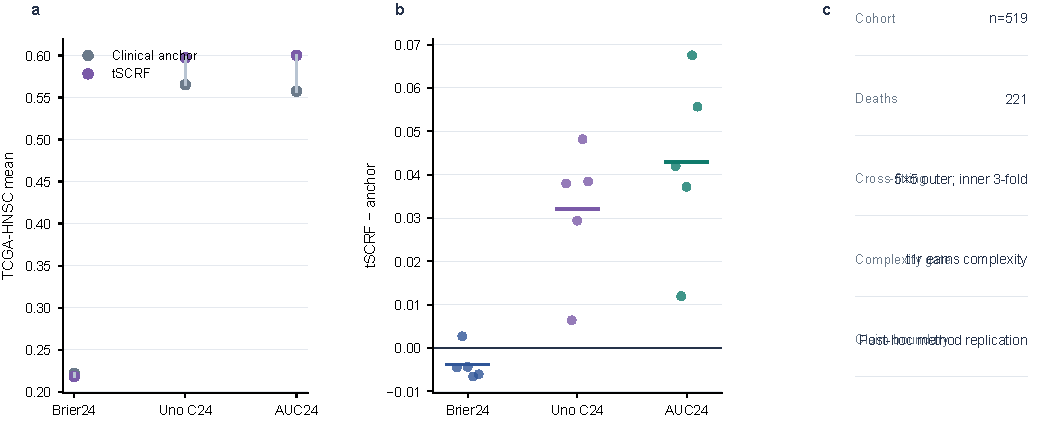
\includegraphics[width=\textwidth]{figures/extended_data_figure3_t1r_transcriptome_replication.pdf}
\caption{\textbf{Transcriptome SCRF method replication in TCGA-HNSC.} \textbf{a}, Mean anchor and tSCRF performance. \textbf{b}, Seed-level tSCRF$-$anchor differences. \textbf{c}, Cohort role and claim label. Discrimination improved in all five seeds.}\label{fig:supp_t1r}
\end{figure*}

A single tSCRF model fitted to the complete TCGA-HNSC development cohort showed favourable Brier and discrimination changes in both GEO cohorts (Table~\ref{tab:supptable8} and Fig.~\ref{fig:supp_geo}). In GSE65858, Uno C increased from 0.583694 to 0.645818. In GSE41613, the applied clinical anchor had no cross-patient variation, whereas tSCRF restored patient-level ordering, with Harrell C 0.626361 and 24-month AUC 0.634011. Calibration slopes above one indicate compressed predicted-risk dispersion, making cohort-level recalibration a constructive next step for prospective absolute-risk reporting.

\begingroup
\scriptsize
\setlength{\tabcolsep}{3pt}
\begin{longtable}{>{\raggedright\arraybackslash}p{0.31\textwidth}rrr}
\caption{GEO transcriptome characterization}\label{tab:supptable8}\\
\toprule
Cohort and metric & Clinical anchor & tSCRF & Difference\\
\midrule
\endfirsthead
\multicolumn{4}{l}{\itshape Table S9 continued from previous page}\\
\toprule
Cohort and metric & Clinical anchor & tSCRF & Difference\\
\midrule
\endhead
\bottomrule
\endlastfoot
\multicolumn{4}{l}{\textbf{GSE65858 (n=244; 78 events)}}\\
IPCW Brier at 24 months & 0.195207 & 0.195070 & $-0.000137$\\
Harrell C & 0.581806 & 0.644868 & $+0.063062$\\
Uno C at 24 months & 0.583694 & 0.645818 & $+0.062123$\\
Time-dependent AUC at 24 months & 0.588972 & 0.650733 & $+0.061762$\\
Calibration-in-the-large & $-0.763793$ & $-0.831959$ & $-0.068166$\\
Calibration slope & 1.707442 & 1.941562 & $+0.234120$\\
\multicolumn{4}{l}{\textbf{GSE41613 (n=97; 51 events)}}\\
IPCW Brier at 24 months & 0.265712 & 0.258607 & $-0.007104$\\
Harrell C & 0.500000 & 0.626361 & $+0.126361$\\
Uno C at 24 months & 0.500000 & 0.616039 & $+0.116039$\\
Time-dependent AUC at 24 months & 0.500000 & 0.634011 & $+0.134011$\\
Calibration-in-the-large & $-0.273717$ & $-0.264792$ & $+0.008925$\\
Calibration slope & -- & 1.939018 & --\\
\end{longtable}
\endgroup

\begin{figure*}[t]
\centering
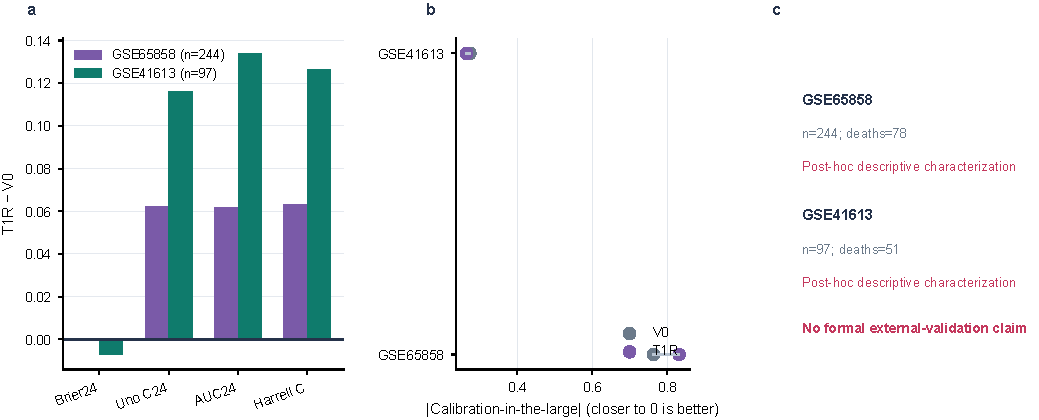
\includegraphics[width=\textwidth]{figures/extended_data_figure4_geo_t1r_characterization.pdf}
\caption{\textbf{GEO cross-platform characterization of transcriptome SCRF.} \textbf{a}, tSCRF$-$anchor differences in GSE65858 and GSE41613. \textbf{b}, Absolute calibration-in-the-large error. \textbf{c}, Cohort sizes and evidence role. A single frozen tSCRF fit retained favourable discrimination changes across platforms.}\label{fig:supp_geo}
\end{figure*}

\begin{figure*}[t]
\centering
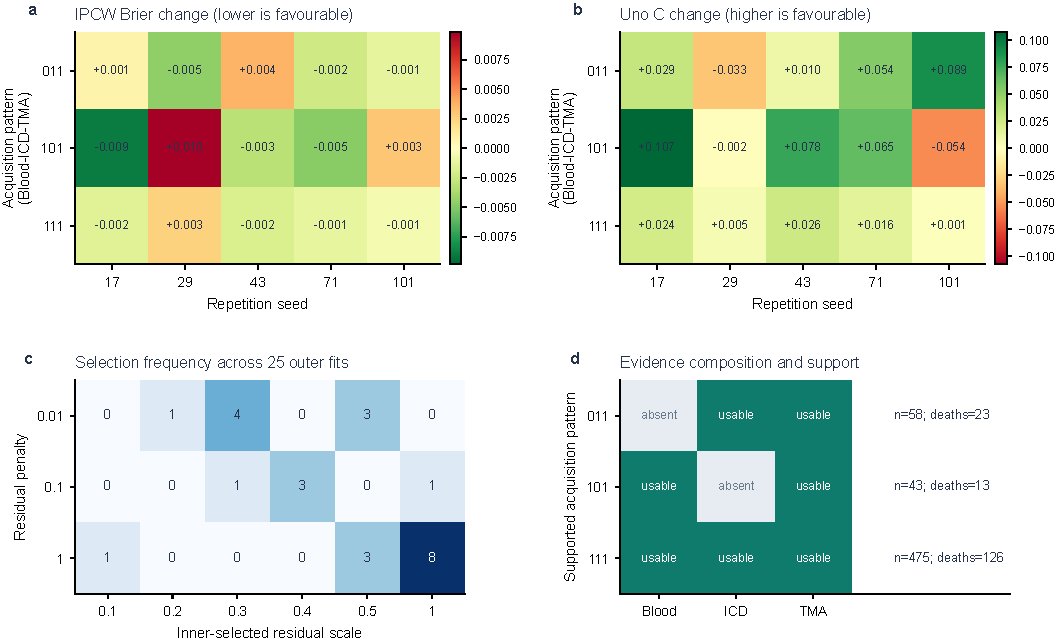
\includegraphics[width=0.96\textwidth]{figures/extended_data_figure5_evidence_pattern_landscape.pdf}
\caption{\textbf{Evidence-pattern and shrinkage-selection landscape.} \textbf{a,b}, Seed-level SCRF--CAM changes in IPCW Brier score and Uno C for the three acquisition patterns meeting the prespecified support criterion. Green denotes a favourable direction for the displayed metric. \textbf{c}, Joint frequency of residual-penalty and residual-scale selections across 25 outer fits. \textbf{d}, Blood--ICD--TMA composition and support of the three evaluable patterns. All panels are generated from aggregate audits; rare patterns remain descriptive only.}\label{fig:supp_pattern_landscape}
\end{figure*}

\section*{S16~Published-method benchmark diagnostics}
The U9--U10 benchmark was added to place SCRF against recognizable published survival algorithms and the fusion-family controls used by recent 2026 missing-modality studies, rather than only against its clinical anchor and internal degradations. All 15 rows in the main benchmark table used five complete repeated OOF prediction sets over the same 610 patients. Neither benchmark accessed confirmation outcomes or altered SCRF. Method-specific calibration summaries are reported here because discrimination and probability-scale accuracy are distinct properties (Table~\ref{tab:supptable9} and Fig.~\ref{fig:supp_comparator_landscape}). The DeepSurv and DeepHit calibration-slope regressions were numerically unstable because their OOF risks were highly dispersed and should not be interpreted as calibrated absolute-risk estimators in this cohort.

\begingroup
\footnotesize
\setlength{\tabcolsep}{2pt}
\begin{longtable}{p{3.0cm}ccc}
\caption{U9--U10 calibration and runtime diagnostics}\label{tab:supptable9}\\
\toprule
Method & \makecell{Calibration-in-\\the-large} & \makecell{Calibration\\slope} & \makecell{Runtime per\\repetition (s)}\\
\midrule
\endfirsthead
\multicolumn{4}{l}{\itshape Table S10 continued from previous page}\\
\toprule
Method & \makecell{Calibration-in-\\the-large} & \makecell{Calibration\\slope} & \makecell{Runtime per\\repetition (s)}\\
\midrule
\endhead
\midrule
\multicolumn{4}{r}{\itshape Continued on next page}\\
\endfoot
\bottomrule
\endlastfoot
Clinical Cox PH & $+0.0401$ (0.0080) & 0.7422 (0.0540) & 0.65\\
Elastic-net Cox & $-0.0185$ (0.0227) & 1.0089 (0.4623) & 0.58\\
Random survival forest & $+0.0135$ (0.0098) & 1.5507 (0.0711) & 5.62\\
Gradient boosting survival & $-0.0116$ (0.0029) & 1.9186 (0.1631) & 1.80\\
XGBoost-Cox & $+0.0384$ (0.0250) & 0.7204 (0.0319) & 0.79\\
DeepSurv & $+0.9428$ (0.2685) & unstable ($>10^{10}$) & 5.60\\
DeepHit & $+0.8460$ (0.2784) & unstable ($>10^{10}$) & 8.27\\
MultiSurv, adapted & $+0.0637$ (0.0445) & 0.4767 (0.0817) & 3.33\\
Early feature fusion, adapted & $-0.5974$ (0.0663) & 0.7027 (0.0843) & 1.32\\
Late decision fusion, adapted & $-1.1033$ (0.0590) & 0.9304 (1.0115) & 1.99\\
Masked attention fusion, adapted & $-0.0782$ (0.0468) & 1.8012 (0.3606) & 2.50\\
Bilinear interaction fusion, adapted & $+0.0668$ (0.0447) & 1.1537 (0.0999) & 3.04\\
Missing-aware intermediate fusion, adapted & $-0.0918$ (0.0450) & 0.1587 (0.0949) & 2.94\\
Heterogeneous aligned fusion, adapted & $-0.0525$ (0.0603) & 0.7723 (0.5607) & 5.17\\
PATTERN-Surv-HN (SCRF) & $-0.0169$ (0.0198) & 0.8513 (0.1693) & --\\
\end{longtable}
\endgroup

Values are mean (s.d.) across five repetitions. Runtimes cover the five-fold U9 or U10 prediction pass for each repetition on the local CPU environment and are descriptive, not hardware-independent complexity measures. SCRF runtime was not recomputed because both benchmarks reused the immutable internal V1R out-of-fold artifact.

\begin{figure*}[t]
\centering
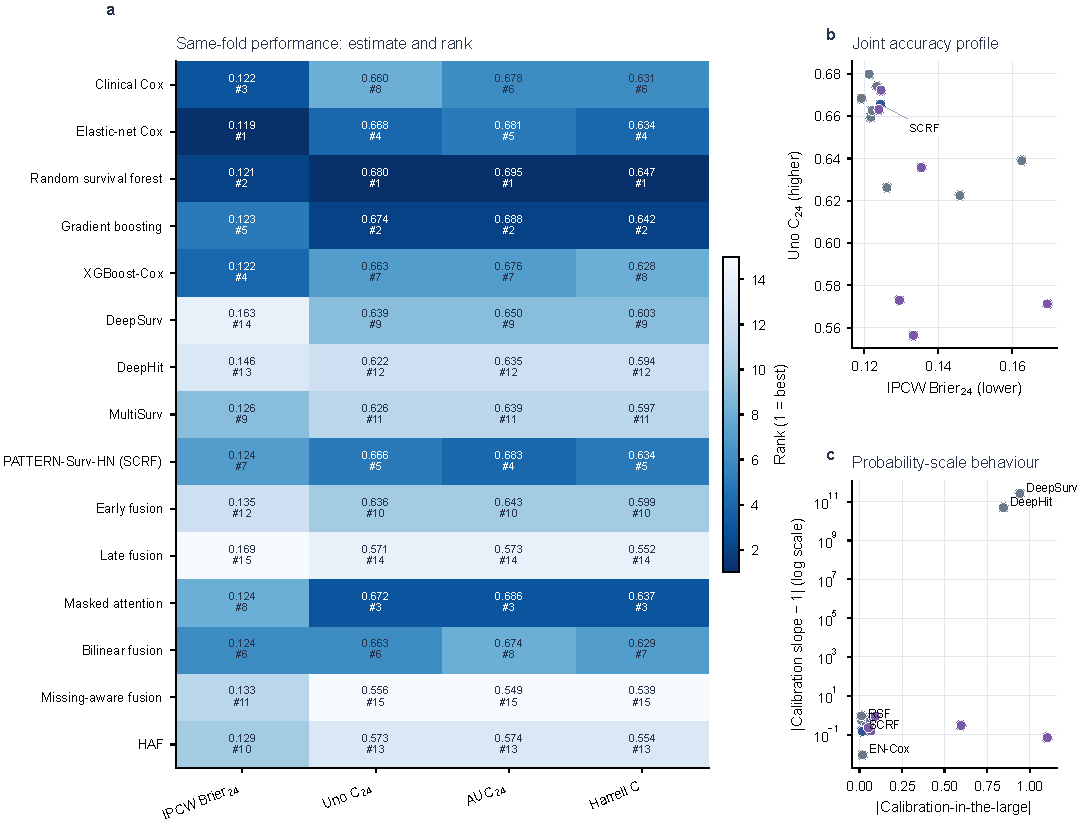
\includegraphics[width=0.96\textwidth]{figures/extended_data_figure6_published_comparator_landscape.pdf}
\caption{\textbf{Published-method performance and calibration landscape.} \textbf{a}, Same-fold mean estimates and within-metric ranks for all fourteen literature-defined comparators and PATTERN-Surv-HN SCRF; rank 1 is best. \textbf{b}, Joint IPCW Brier--Uno C profile. \textbf{c}, Absolute calibration-in-the-large and calibration-slope error; the logarithmic ordinate accommodates the unstable DeepSurv and DeepHit slopes without suppressing them. Blue denotes SCRF, purple denotes recent fusion-family adaptations and grey denotes established comparators. This is a post-hoc development benchmark, not a locked superiority analysis.}\label{fig:supp_comparator_landscape}
\end{figure*}

\section*{S17~Reproducibility and artifact governance}
The formal SCRF development out-of-fold artifact (internal identifier V1R) had SHA256 \hashid{E43BB6C0D8E2C7F9C8B22A9C416AD752109B926A8526273D88811458CD73BCE0}. The confirmation protocol SHA256 was \hashid{1E134D30557D1CC153997F6EBB79E99C2E160F85A9F94BF3BBDD81C2C588BDED}, and the locked prediction artifact SHA256 was \hashid{E5DA83BDB3BB97C3488687C78CCF166FBD03059619DD0690E2767CAF8F393FCF}. Two CAM reruns (internal identifier V0) produced identical out-of-fold hashes.

Aggregate sources included \path{U5R7_V1R_beta09_logloss_bridge_candidate/selected_bridge_aggregate_results.json}, \path{U6R1_patient_level_router_aggregation_exploration/u6r1_aggregate_results.json}, \path{U7R2_RADCURE_external_characterization/u7r2_radcure_external_characterization_aggregate_results.json}, \path{U8_T1R_transcriptome_residual_shrinkage/aggregate_t1r_transcriptome_development_cv_audit.json}, \path{U8E_T1R_external_characterization/aggregate_t1r_external_characterization_audit.json}, \path{results/metrics/pattern_surv_hn/U9_published_comparator_benchmark/aggregate_u9_published_comparator_benchmark_audit.json} and \path{results/metrics/pattern_surv_hn/U10_recent_comparator_benchmark/aggregate_u10_recent_comparator_benchmark_audit.json}. The U9 audit SHA256 was \hashid{ABEC65258668E34AE91FAFFADAF2FCE6C5D6F6CAF4097E6CAF53D18AB7B74050}; its main-table CSV SHA256 was \hashid{B452C7A32EB7ED6303DBABF315D78A2374AABFD132662A3FE8CCB455A7702DDD}. The expanded U10 audit SHA256 was \hashid{AD005361FEF53AB25F93B73C6C4D5992741961CA0D0E8D71224CFDF4033B7142}; its main-table CSV SHA256 was \hashid{BA6C0B9EC1AAAD86F78D40B67B1486C42375156AD4E3F5C5DFBA7ABE77839129}. Figure provenance is recorded in \path{figures/figure_manifest.json}; publication figures are generated by \path{generate_figures.py}.

Cohorts, preprocessing and stage definitions were configuration controlled. Repetition seeds were 17, 29, 43, 71 and 101. Each stage recorded analysis label, prior outcome access, tuning status and artifact integrity. Patient identifiers and patient-level predictions were excluded from version control; publication-facing tables and figures were generated from aggregate metrics, manifests and audits. This governance allows every central number to be traced to a frozen artifact without redistributing restricted patient-level predictions.

\bibliography{references}
\end{document}
